\section{Project Results}
\label{sec:results}
This section presents the results of the person localization system implemented in the thesis project work. This includes a diverse range of experiments relevant for the objectives of this thesis. The results are discussed with regards to their implications and significance in the context of the research questions and objectives outlined in Section \ref{sec:research_questions}, and in the broader context of the field.

\paragraph{Metrics and Notations}
The tables \ref{tab:APs_fine_tuning}, \ref{tab:larger_test_set}, and \ref{tab:APs_imagesize} shows the AP scores when the models are evaluated with "COCO AP". This means to only average over 10 IoU thresholds, while keeping the confidence threshold fixed. As mentioned in Section \ref{sec:accuracy_of_model_inferences}, this has been the de-facto method of calculating average precision since its introduction with the COCO dataset challenge in 2017. The confidence threshold is kept fixed at 0.5, which is the default value for the COCO challenge. In this thesis, we denote COCO AP as \textit{AP}, and the other method of calculating average precision where both the IoU and COCO thresholds are varied is denoted as \textit{vary-both AP}. 

Additionally, for simplicity, the models that are not fine-tuned are denoted as \textit{standard} models. The weights of these models are directly available for download online. The fine-tuned models are fine-tuned on these standard weights.

\subsection{Object Detection Model Evaluation}
\label{sec:object_detection_model_evaluation}
The characteritics of the dataset partitions allow us to execute several experiments. The experiments are designed to answer the research questions and objectives outlined in Section \ref{sec:research_questions}. Various evaluation jupyter notebooks used in this thesis to evaluate the models are found at \href{github.com/hallvaeb/masterthesis}{this github}. 

\subsubsection{Fine-Tuning On \textit{Consistent-2}, Testing On \textit{Consistent-1}}
The test-set should cover as many situations as possible that the detector may face after deployment, and be as diverse as possible. The \textit{Consistent-1} and \textit{Consistent-2} are similar, but have some minor differences (differences were detailed in Section \ref{sec:consistent_datasets_differences}). These differences may affect the results, and obscure whether the results are due to the differences in the dataset sizes or the differences in the dataset content. Regardless, using a smaller test-set reduces validity of the results. It is necessary, however, when a portion of the test-set is needed for fine-tuning. Since the same data must not be used for training and validation or testing, the models displayed in \ref{tab:APs_fine_tuning}, which were fine-tuned on \textit{Consistent-2}, are only evaluated on \textit{Consistent-1}.

\begin{table}[H]
    \centering
    \renewcommand{\arraystretch}{1.5} % Increase vertical padding
    \setlength{\tabcolsep}{1em}
    \begin{tabular}{|l|c|c|c|c|}
        \hline
        \rowcolor{gray!25}
        \textbf{Model} & \textbf{AP50} & \textbf{AP75} & \textbf{AP90} & \textbf{mAP50-95} \\ \hline
        Standard             & 0.982 & 0.959 & 0.935 & 0.959 \\ \hline 
        Fine-Tuned 5 Epochs  & 0.969 & 0.881 & 0.645 & 0.815 \\ \hline
        Fine-Tuned 10 Epochs & 0.976 & 0.889 & 0.660 & 0.823 \\ \hline
        Fine-Tuned 20 Epochs & 0.971 & 0.883 & 0.648 & 0.821 \\ \hline
    \end{tabular}
    \caption{Comparison of Various YOLOv9 Models Fine-Tuned on Consistent-2 (465 images) and Evaluated on Consistent-1 (292 images)}
    \label{tab:APs_fine_tuning}
\end{table}

The scores in Table \ref{tab:APs_fine_tuning} shows the standard model outperformed the fine-tuned models. This may be due to the low number of epochs they are trained for. Another reason to the fine-tuned models performing poorly may be due to the simplicity of the dataset. The worsened results by fine-tuning is partly unexpected, but may be due to catastrophic forgetting, which was tried to be avoided by freezing the backbone of the YOLO models. More discussions regarding the results are found in Section \ref{sec:table_discussion}, which displays similar results. We will first further investigate the characteristics of the test-set.

\subsubsection{Test-Set Exploration}
\label{sec:larger_test_set}
The following table presents the performance metrics of YOLOv3 and YOLOv9 on different test sets composed from the images of the FIMUS dataset. These models are pre-trained with COCO images, and was never trained nor fine-tuned with FIMUS data. The table highlights the Average Precision (AP50-95) and Average Recall (AR50-95) metrics across these test sets.

\begin{table}[H]
    \centering
    \renewcommand{\arraystretch}{1.5} % Increase vertical padding
    \setlength{\tabcolsep}{1em}
    \begin{tabular}{|c|l|c|c|c|c|}
        \hline
        \rowcolor{gray!25}
        \textbf{Model} & \textbf{Test Set} & \textbf{Sample} & \textbf{Max Persons} & \textbf{AP50-95} & \textbf{AR50-95} \\ \hline
		YOLOv3 & Consistent-1  & n=292 & 4 & 0.826 & 0.727 \\ \hline
		YOLOv3 & Consistent-2  & n=465 & 2 & 0.795 & 0.847 \\ \hline
		YOLOv3 & Consistent    & n=757 & 4 & 0.681 & 0.734 \\ \hline
		YOLOv3 & Inconsistent  & n=2637& 1 & 0.840 & 0.851 \\ \hline
        YOLOv3 & FIMUS dataset & n=3394& 4 & 0.770 & 0.801 \\ \hline
        YOLOv9 & Consistent-1  & n=292 & 4 & \textbf{0.959} & 0.826 \\ \hline
		YOLOv9 & Consistent-2  & n=465 & 2 & 0.910 & 0.949 \\ \hline
		YOLOv9 & Consistent    & n=757 & 4 & 0.945 & 0.865 \\ \hline
		YOLOv9 & Inconsistent  & n=2637& 1 & 0.929 & \textbf{0.971} \\ \hline
        YOLOv9 & FIMUS dataset & n=3394& 4 & 0.936 & 0.921 \\ \hline
    \end{tabular}
    \caption{Comparison of YOLOv3 and YOLOv9 on Various Quality Test Data}
    \label{tab:larger_test_set}
\end{table}

Like previous research has shown, YOLOv9 outperforms YOLOv3. The YOLOv3 model was included in this experiment to see if it would outperform its successor for any of the data, which it did not. 

The consistent test sets (\textit{Consistent-1}, \textit{Consistent-2}, \textit{Consistent}) represent subsets within the \textit{Consistent} partition. Analyzing the results on these sets shows some variability. For instance, the AP50-95 for YOLOv9 drops from 0.959 in \textit{Consistent-1} to 0.945 in the combined Consistent set, while the AR50-95 increases from 0.826 to 0.865. This suggests that even within high-quality images, the model's evaluation will vary significantly based on which evaluation metric is used, and on which test-set. The increase of AP and simultaneus decrease in AR for the same confidence thresholds means that the differences stems from the variation of the dataset partitions. 

\textit{Consistent-1} has higher precisions and lower recalls than \textit{Consistent-2}. This means that the persons in \textit{Consistent-1} are more often missed. This may be due to the additional occlusions that are introduced with the increased number of persons compared to \textit{Consistent-2}, making it harder to detect all persons in the image. 

Generally, the models perform very well, achieving scores far beyond the scores typically achieved on bigger, generic and possibly harder to infer on datasets. This shows our choice in machine learning architecture for the given environment and scale is has been successful\footnote{The high scores could also indicate something has gone wrong in our evaluation pipeline. This is considered unlikely, however, after having looked at images from the inferences and verified a lot of the inferences are indeed correct.}. 

Finally, this evaluation of the various test sets serves as a demonstration of the accuracies of YOLOv9 for the specific environment, which surpasses the accuracies of the same model on the COCO dataset. This is further demonstrated and underscored in the following results.

\subsubsection{Input Image Size}
\label{sec:input_image_size}
We experimented with the input image size for model inference with the standard YOLOv9 to find the optimal value. 320, 640 and 1280 were tested. The input image size affects accuracy and inference latency of the models. The inferences were performed using an 8-core AMD® Ryzen 7 4700u CPU with 16GiB RAM\footnote{The inference machine hardware specification is mentioned here, and not in the methodology section, as this is the only place in the thesis where speed is discussed and the inference machine hardware is of relevance. The machine's hardware does not affect inference accuracy.}, resulting in higher inference latencies than what are usually reported for similar models. In addition to the hardware, other simultaneuos tasks on the computer may affect inference latency. Therefore, no other user input was given during these model inference runs. However, background processes and other programs were not terminated during the process, so the numbers are only not valid outside this thesis. More valid results could have been achieved by running the inference many times and taken the average inference latency. 

The weights file also affects the inference latency. The YOLOv9 is released with three sets of pre-trained weights. These are called yolov9-m, -c, and -e (as of 03.06.2024). The results of Table \ref{tab:APs_imagesize} were achieved using the yolov9-\textit{e} weights. 

\begin{table}[H]
    \centering
    \renewcommand{\arraystretch}{1.5}
    \setlength{\tabcolsep}{1em}
    \begin{tabular}{|l|c|c|c|}
        \hline
        \rowcolor{gray!25}
        \textbf{Model} & \textbf{Input Image Size}& \textbf{mAP50-95} & \textbf{Inference Latency} \\ \hline
        YOLOv9          & 320  & 0.820 & 302ms  \\ \hline
        YOLOv9          & 640  & 0.945 & 840ms  \\ \hline
        YOLOv9          & 1280 & 0.877 & 3336ms \\ \hline
    \end{tabular}
    \caption{Comparison of Yolov9 Models With Various Input Image Sizes Evaluated on \textit{Consistent}}
    \label{tab:APs_imagesize}
\end{table}

Table \ref{tab:APs_imagesize} reveals the effects of input image size on model performance. Performing model inference with an input image size of 1280 was hypothesized to augment the accuracies, but this was not the case in our experiment. Introducing a much higher inference latency and poorer performance than of the 640 image size, the 1280 is clearly the worst option. This is likely due to the scale of the persons in the FIMUS Consistent dataset partition, which does not necessitate a higher input image size than 640. Inferring with size 320 may be a viable option in applications where speed is important.  

\subsubsection{Model Average Precisions on Consistent Dataset}
The models were evaluated using both COCO AP \textit{and} Vary-Both AP metrics, increasing reproducibility as future developments and evaluations may freely choose between the two methods. The rankings of the models are similar for both evaluation metrics, demonstrating that the choice of evaluation metric is not detrimental to the process of finding the optimal model for a deployment scenario. The results are discussed in depth in following paragraphs.

\paragraph{COCO AP}
The AP and the AR of the models varied with number of epochs they were fine-tuned for. The scores are displayed in Figure \ref{fig:plot_AP_COCO}.

\begin{figure}[H]
    \centering
    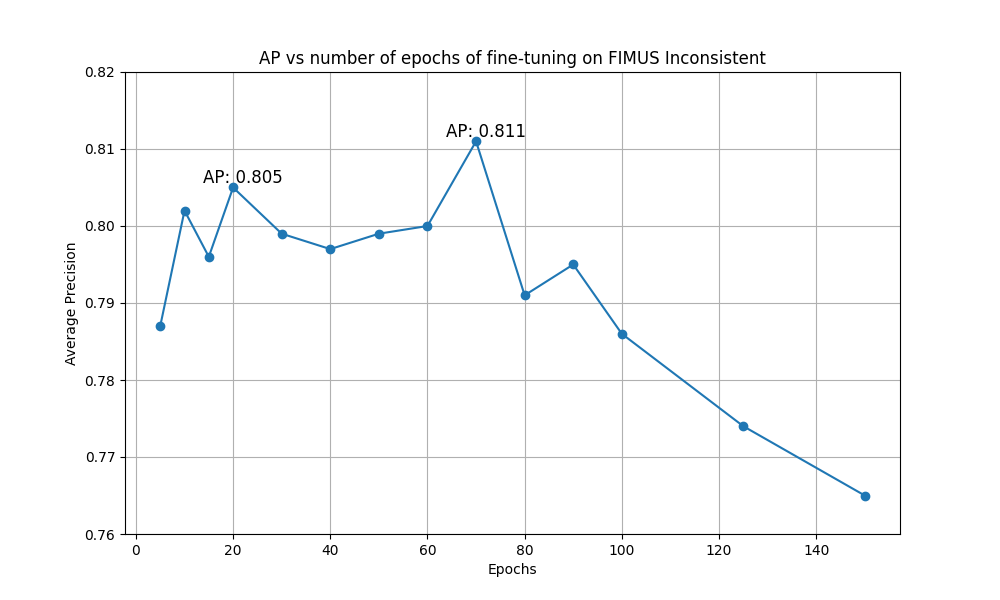
\includegraphics[width=\textwidth]{Images/Analytics/plot_AP_coco.png}
    \caption{Average Precisions Over Number of Epochs Fine-Tuned on Inconsistent}
    \label{fig:plot_AP_COCO}
\end{figure}

The model achieving the best average precision was fine-tuned for 70 epochs. Notably, we observed a local maximum at 20 epochs. Had we not continued training past 60 epochs, we would not have known the model could improve at 70 epochs. The average precision scores were also calculated and are displayed in the graph of Figure \ref{fig:plot_AR}.

\begin{figure}[H]
    \centering
    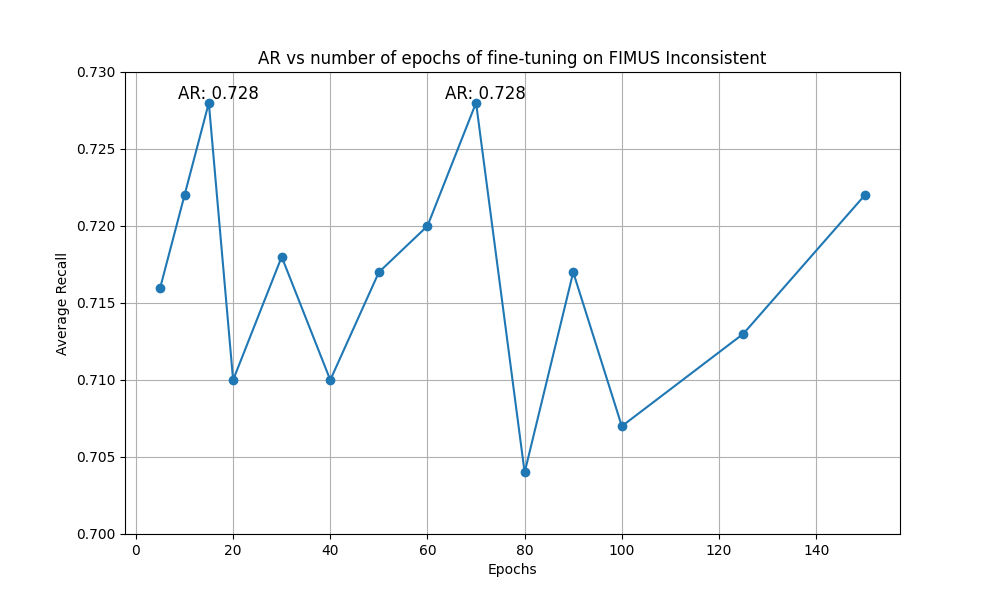
\includegraphics[width=\textwidth]{Images/Analytics/plot_AR.png}
    \caption{Average Recalls Over Number of Epochs Fine-Tuned on Inconsistent}
    \label{fig:plot_AR}
\end{figure}

We observed that the best models regarding average recall were achieved after 15 and 70 epochs. Considering both AP and AR for the models, it is clear that fine-tuning the model for 70 epochs produced the highest-scoring fine-tuned model. A comparison of this model and all other models on the FIMUS Consistent dataset partition is displayed in Table \ref{tab:APs_models_COCO}.

\begin{table}[H]
    \centering
    \renewcommand{\arraystretch}{1.5}
    \setlength{\tabcolsep}{1em}
    \begin{tabular}{|l|c|c|c|c|}
        \hline
        \rowcolor{gray!25}
        \textbf{Model} & \textbf{AP50} & \textbf{AP75} & \textbf{AP50-95} & \textbf{AR50-95} \\ \hline
        YOLOv9-m Standard         & 0.957 & 0.908 & 0.865 & 0.716 \\ \hline
        YOLOv9-c Standard         & 0.932 & 0.885 & 0.845 & 0.747 \\ \hline
        YOLOv9-e Standard         & 0.972 & 0.949 & \textbf{0.945} & \textbf{0.865} \\ \hline
        YOLOv9 CrowdHuman 5ep     & 0.968 & 0.916 & 0.834 & 0.692 \\ \hline
        YOLOv9 CrowdHuman 10ep    & 0.964 & 0.914 & 0.831 & 0.702 \\ \hline
        YOLOv9 Inconsistent 70ep  & 0.954 & 0.867 & 0.811 & 0.728 \\ \hline
        YOLOv9 PRW 5ep            & 0.802 & 0.681 & 0.605 & 0.389 \\ \hline
        YOLOv9 PRW 10ep           & 0.969 & 0.856 & 0.721 & 0.455 \\ \hline
        YOLOv3                    & 0.804 & 0.742 & 0.681 & 0.734 \\ \hline
        DETR-50 Conf 0.50         & 0.404 & 0.347 & 0.307 & 0.675 \\ \hline
        DETR-50 Conf 0.99         & 0.776 & 0.711 & 0.624 & 0.549 \\ \hline
        DETR-101 Conf 0.50        & 0.606 & 0.535 & 0.468 & 0.689 \\ \hline
        DETR-101 Conf 0.99        & 0.818 & 0.762 & 0.665 & 0.559 \\ \hline
    \end{tabular}
    \caption{Models APs on \textit{Consistent} (757 images)}
    \label{tab:APs_models_COCO}
\end{table}

\paragraph{Results Discussion}
\phantomsection
\label{sec:table_discussion}
These results show no accuracy improvements from fine-tuning. The standard models performed best on the Consistent dataset. The results indicate that freezing the backbone and fine-tuning the head on inconsistent, highly relevant data was a destructive practice. A notable discovery was the already high scores the YOLOv9 achieves on the \textit{Consistent} (and the rest of the FIMUS dataset). \citeauthor{wang2024yolov9} report a score of 0.556 on the COCO dataset, which is substantially lower than the scores we achieved on FIMIST Consistent. This may seem odd, as the model weights are pre-trained on COCO data, which should be more similar to the test data for the same dataset. However, as discussed in the section introducing the COCO dataset (see \ref{sec:dataset_COCO}), it is a very difficult, highly diverse dataset. In our Consistent dataset, if a model is able to correctly infer one image, it is likely to also infer correctly on the rest of the images because they are very similar in nature.

Out of the fine-tuned models, the YOLOv9 model trained on the CrowdHuman dataset achieved some of the highest scores. This is not unexpected: The dataset contains a lot of diversity and probably more instances of humans to learn from than the Inconsistent FIMUS dataset. The models that were fine-tuned on Inconsistent were trained for a tenfold more epochs to try to make up for this fact, but the accuracies failed to improve. These results indicate that rather than producing a sub-optimal specialized dataset for fine-tuning a model, the better option may be to use a larger and better dataset.

Should the positioning of the bounding boxes be of less importance, we see that fine-tuning on the PRW dataset is still a better option than fine-tuning on our FIMUS Inconsistent dataset partition. This is revealed by the AP50 score of 0.969 after just 10 epochs, while training on FIMUS Inconsistent did not achieve similar results in its 150 epochs of training.

The attentive reader may have noticed the Football Players Detection Fine-Tuned models are not included in the results presented in Table \ref{tab:APs_models_COCO}. This is because both the 5 epochs and 10 epochs model both completely missed the persons in the aquarium. This could have been due to the difference in scale, resulting in a fine-tuned model not able to predict the humans in the aquarium setting. A review of the labels indicate that the model had close to no inferences with a confidence score higher than 0.1, and the highest confidence at 0.425. An attempt was made to improve the scores by detecting at confidence threshold 0.001, then normalizing the detections, but the poor model performances were not salvageable. An example from the labeled images is displayed in figure \ref{fig:football_unsalvageable}. Interestingly, it does not infer the roof lamp to be a person, like we saw with the standard YOLOv9.

\begin{figure}[H]
    \centering
    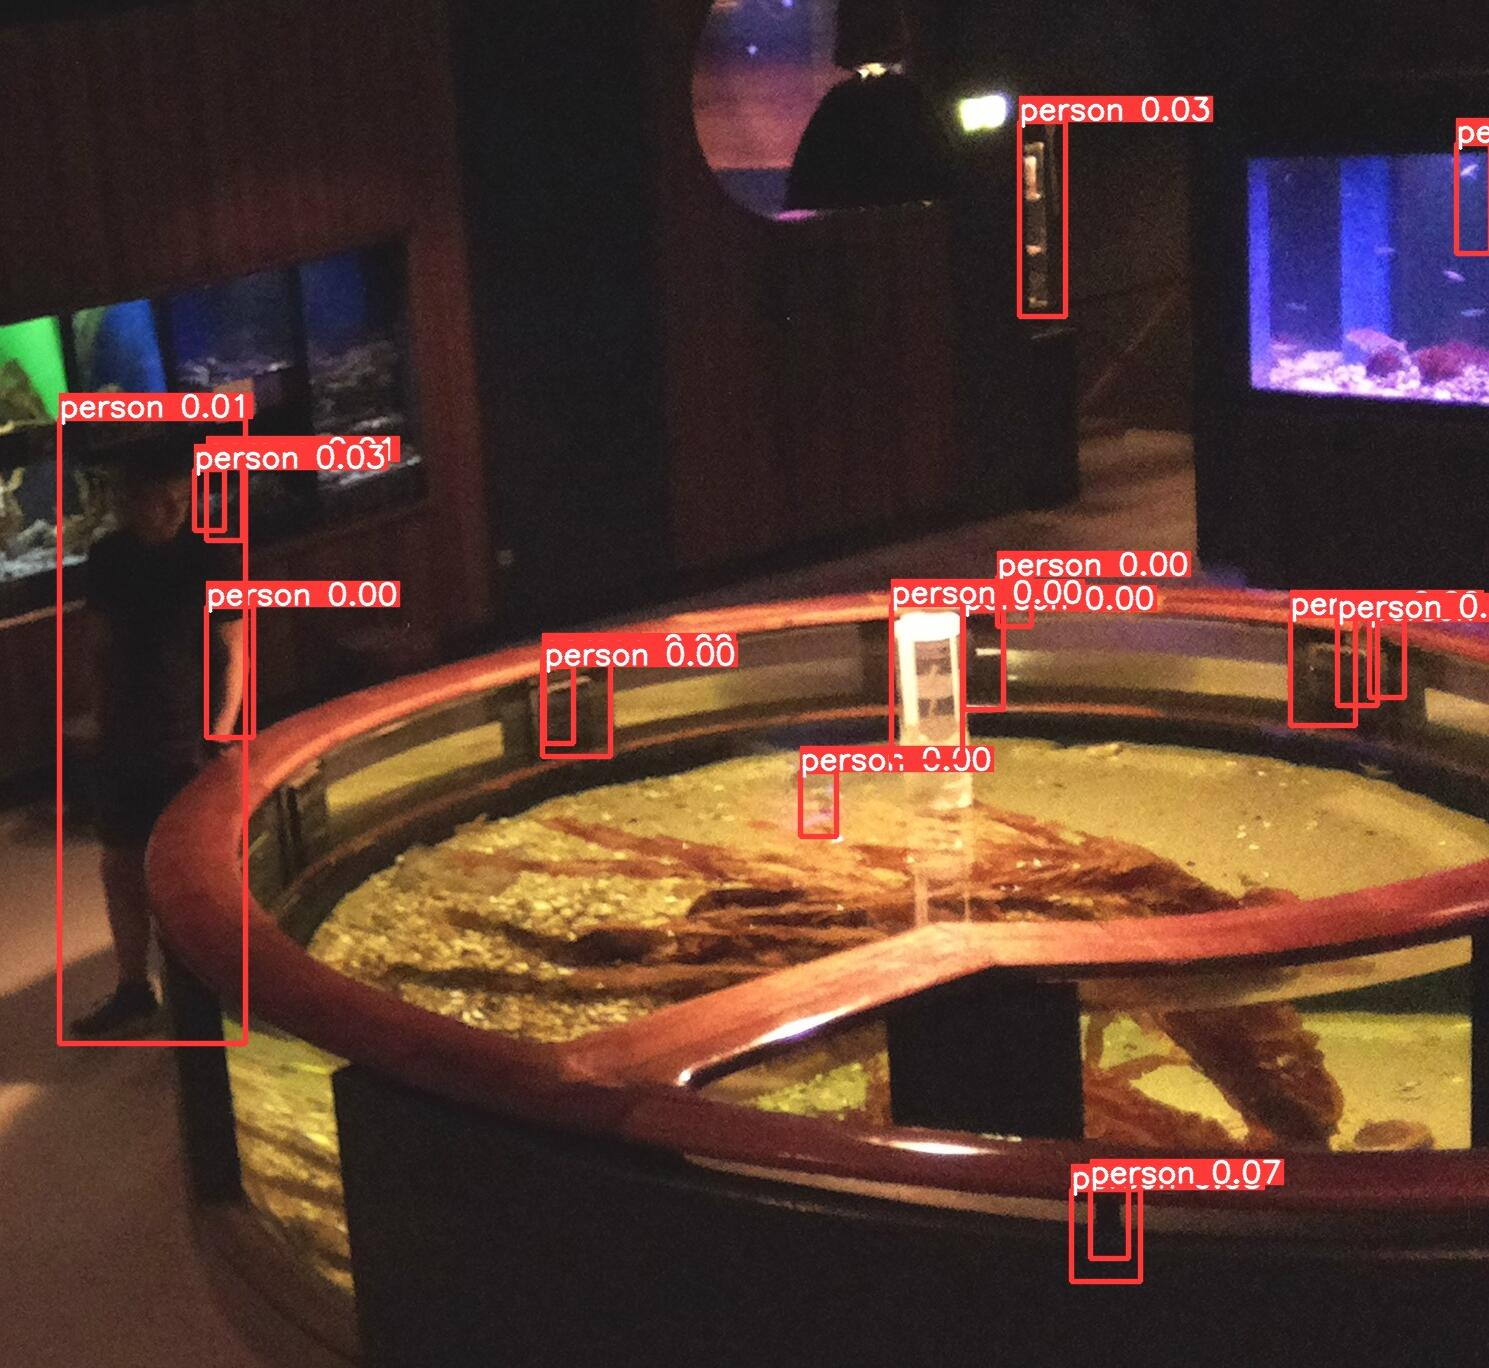
\includegraphics[width=0.6\textwidth]{Images/Results/football_unsalvageable.jpg}
    \caption{Example Image of the Unsalvageable Football Players Model Inferences}
    \label{fig:football_unsalvageable}
\end{figure}

The reasons for this model failure was due to a mistake made when freezing the backbone. Only the 10 first layers were frozen, instead of all 28, resulting in a model that has suffered from the catastrophic forgetting problem which, as mentioned, is especially prevalent in tiny ML applications. The model would then have to be retrained, for which there were no resources left to do in this thesis project.

The fixed confidence threshold was raised for the DETR models since they report vastly higher confidence scores than many other model architectures. Therefore, the confidence scores were fixed at 0.99. A comparison of the inference latencies of the models were not conducted, as the YOLO model is still clearly the better option. We see, however, that this raise in confidence threshold naturally also results in a reduced AR score for the models. For the calculations of Vary Both AP, the confidence threshold was varied similar to every other model.

Another surprising result from Table \ref{tab:APs_models_COCO} is the YOLOv9-m performance relative to the larger weights of c and e. These letters correspond to different pre-trained weights, with various number of parameters. The converted version\footnote{There's also converted vs not converted models. The reparameterization functionality to convert a model consists of trimming layers meant to speed up and augment model training, which is not needed for running model inference. The converted models achieve the same results but with lower inference latency, smaller size. They should not, however, be used for fine-tuning.} of YOLOv9-e weight file has a size of 117.2MB, YOLOv9-c and -e fills only respectively 51.4MB and 40.7MB of space.

\paragraph{Vary-Both AP}
Figure \ref{fig:plot_AP_both} displays how the AP of the models varied with the number of epochs. Equally to the COCO AP, the best model was the standard YOLOv9-e. We recall the Vary-Both AP references to the AP score achieved when evaluating models with a varying IoU threshold of 10 values from 0.50-0.95 \textit{and} confidence threshold from 0.10 to 0.90 in 20 steps.

\begin{figure}[H]
    \centering
    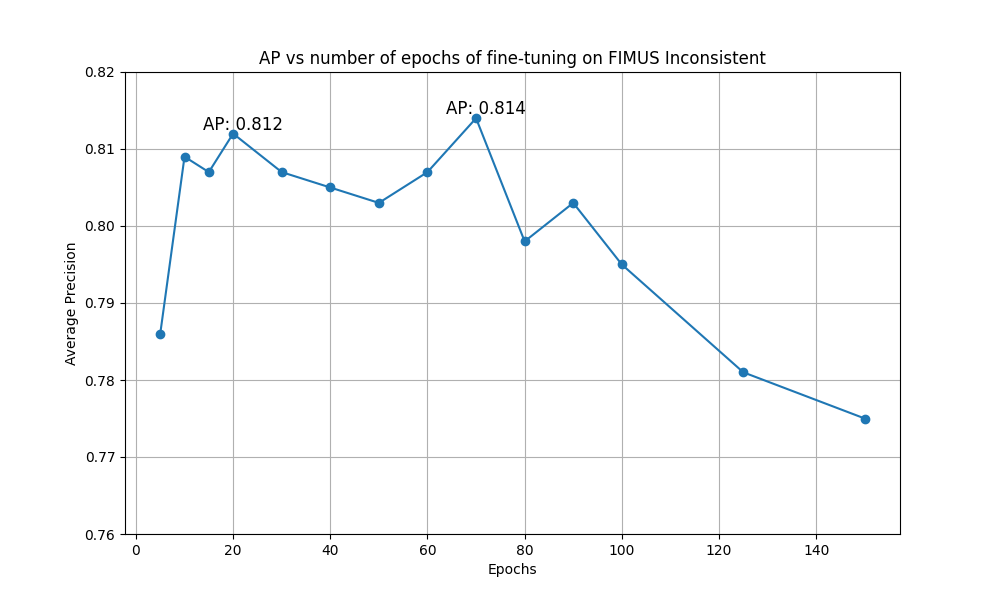
\includegraphics[width=.8\textwidth]{Images/Analytics/plot_AP_both.png}
    \caption{Vary-Both APs Over Number of Epochs Fine-Tuned on Inconsistent}
    \label{fig:plot_AP_both}
\end{figure}

The following table (\ref{tab:APs_models_both}) displays how well the models performed on the Consistent dataset. Similar to the results in Table \ref{tab:APs_models_COCO}, the YOLOv9-e was the most accurate, achieving an AP50-95 of 0.913.

\begin{table}[H]
    \centering
    \renewcommand{\arraystretch}{1.5}
    \setlength{\tabcolsep}{1em}
    \begin{tabular}{|l|c|c|c|c|}
        \hline
        \rowcolor{gray!25}
        \textbf{Model} & \textbf{AP50} & \textbf{AP75} & \textbf{AP90} & \textbf{AP50-95} \\ \hline
        YOLOv9-m Standard                & 0.895 & 0.855 & 0.746 & 0.821 \\ \hline
        YOLOv9-c Standard                & 0.881 & 0.842 & 0.740 & 0.810 \\ \hline
        YOLOv9-e Standard                & 0.942 & 0.918 & 0.876 & \textbf{0.913} \\ \hline
        YOLOv9 on Inconsistent for 20ep  & 0.948 & 0.854 & 0.680 & 0.812 \\ \hline
        YOLOv9 on Inconsistent for 70ep  & 0.948 & 0.867 & 0.674 & 0.814 \\ \hline
        YOLOv9 on PRW for 5ep            & 0.808 & 0.706 & 0.427 & 0.633 \\ \hline
        YOLOv9 on PRW for 10ep           & 0.924 & 0.792 & 0.252 & 0.677 \\ \hline
        YOLOv9 on CrowdHuman for 5ep     & 0.908 & 0.863 & 0.688 & 0.788 \\ \hline
        YOLOv9 on CrowdHuman for 10ep    & \textbf{0.944} & 0.902 & 0.740 & 0.822 \\ \hline
        YOLOv9 on Football for 5ep       & 0.221 & 0.177 & 0.175 & 0.179 \\ \hline
        YOLOv9 on Football for 10ep      & 0.514 & 0.457 & 0.443 & 0.452 \\ \hline
        YOLOv3                           & 0.780 & 0.728 & 0.528 & 0.672 \\ \hline
        DETR ResNet50                    & 0.414 & 0.355 & 0.164 & 0.315 \\ \hline
        DETR ResNet101                   & 0.594 & 0.526 & 0.245 & 0.460 \\ \hline
    \end{tabular}
    \caption{Comparison of Detectors APs on Consistent (757 images), Multiple IoU and Confidence Thresholds}
    \label{tab:APs_models_both}
\end{table}

Table \ref{tab:APs_models_both} includes AP90 instead of AR50-95 to highlight a separate discovery from what is discussed around Table \ref{tab:APs_models_COCO}. We see the standard YOLOv9-e is still the highest scoring model, even when calculating the AP with varying IoU and confidence thresholds as opposed to calculating COCO AP where the confidence is fixed. However, we also notice the YOLOv9 fine-tuned on the CrowdHuman dataset for 10 epochs is better performing than the standard model when the accuracies of the bounding boxes are less strict, i.e. the IoU value is lower. This indicate that our training data may have been imprecise in bounding box placements. Human errors are not uncommon. The YOLOv9-e is best performing not only due to the high precision for IoU threshold at 0.50, but the maintained precision as the IoU threshold is tightened up to the final value of 0.95. This suggests the training data for fine-tuning the models may have been suboptimal in its bouding box placement. 

Another difference from the COCO AP evaluation is that here, the DETR models were also varied from 0.1 to 0.90 in confidence thresholds, resulting in much worse average precisions than when the confidence threshold for these models were fixed at 0.99.

\paragraph{DETR Fixed Confidence Thresholds' Effects on Average Precision}
The poor performances of the DETR models motivated the an investigation of the labels. The DETR models infer with much higher confidences, making the fixed threshold at 0.5 way too low to score well on the COCO metric. An assessment was made thus made to find the optimal confidence level for the model. This was found at 0.991, nearly doubling the AP score from 0.315 to 0.625 for the DETR with a ResNet50 backbone, and improving the score from 0.460 to 0.668 for the model with the more complex ResNet101 backbone.

\begin{table}[H]
    \centering
    \renewcommand{\arraystretch}{1.5}
    \setlength{\tabcolsep}{1em}
    \begin{tabular}{|l|c|c|c|c|}
        \hline
        \rowcolor{gray!25}
        \textbf{Model} & \textbf{AP50} & \textbf{AP75} & \textbf{AP90} & \textbf{mAP50-95} \\ \hline
        DETR ResNet50 Conf  0.50             & 0.414 & 0.355 & 0.164 & 0.315 \\ \hline
        DETR ResNet50 Conf  0.95             & 0.755 & 0.660 & 0.326 & 0.585 \\ \hline
        DETR ResNet50 Conf  0.99             & 0.776 & 0.711 & 0.369 & 0.624 \\ \hline
        DETR ResNet50 Conf  0.991            & 0.773 & 0.713 & 0.373 & 0.625 \\ \hline
        DETR ResNet101 Conf 0.50             & 0.594 & 0.526 & 0.245 & 0.460 \\ \hline
        DETR ResNet101 Conf 0.95             & 0.795 & 0.719 & 0.353 & 0.627 \\ \hline
        DETR ResNet101 Conf 0.99             & 0.818 & 0.762 & 0.408 & 0.665 \\ \hline
        DETR ResNet101 Conf 0.991            & 0.818 & 0.767 & 0.419 & 0.668 \\ \hline
    \end{tabular}
    \caption{APs for DETR When Fixing the Confidence Threshold at Various Values (757 images).}
    \label{tab:DETR_conf}
\end{table}

The results presented in Table \ref{tab:DETR_conf} are in accordance with the results of \citeauthor{carion2020endtoend}. They claim it is performing well on panoptic segmentation, a task where pixel-level detail is important. This is the reason to the confidence values are high for the task of object detection. For the experiments in Table \ref{tab:APs_models_COCO}, a threshold of 0.99 was used instead of 0.991, because experimentally finding the optimal confidence threshold post-inference on a test-set is likely overfitted to the testing data and not so easy to optimize for in a practical setting.

The results of this section are put into a broader context in the Discussion section, see \ref{sec:discussion_broader_context}.

\subsection{Data Visualization}
\label{sec:data_visualization}
The obtained localization data of visitors may be visualized a multiple of ways. The explored methods in this thesis are by creating heat maps and bar charts to visualize the data. 

\subsubsection{Visitor Localization Heat maps}
\label{sec:results_heat maps}
As mentioned in Section \ref{sec:heat_maps}, heat maps are a powerful visualization tool that can provide insights into visitor behavior patterns and engagement levels within a museum or aquarium setting. Heat maps for the month of may are illustrated in \ref{fig:heat_map_final}. These heat map generation code for the two heat maps are identical, apart from one variable: the position where detections are mapped to. In \ref{fig:heat_map_final}a and b, the detections are mapped to the respectively the middle and the bottom center of the detection bounding box. This single modification has the largest difference on the edges of occlusions, such as (for the images in Figure \ref{fig:heat_map_final}) the railing of the fish tank in the center.

\begin{figure}[H]
    \centering
    \begin{subfigure}{0.475\textwidth}
        \centering
        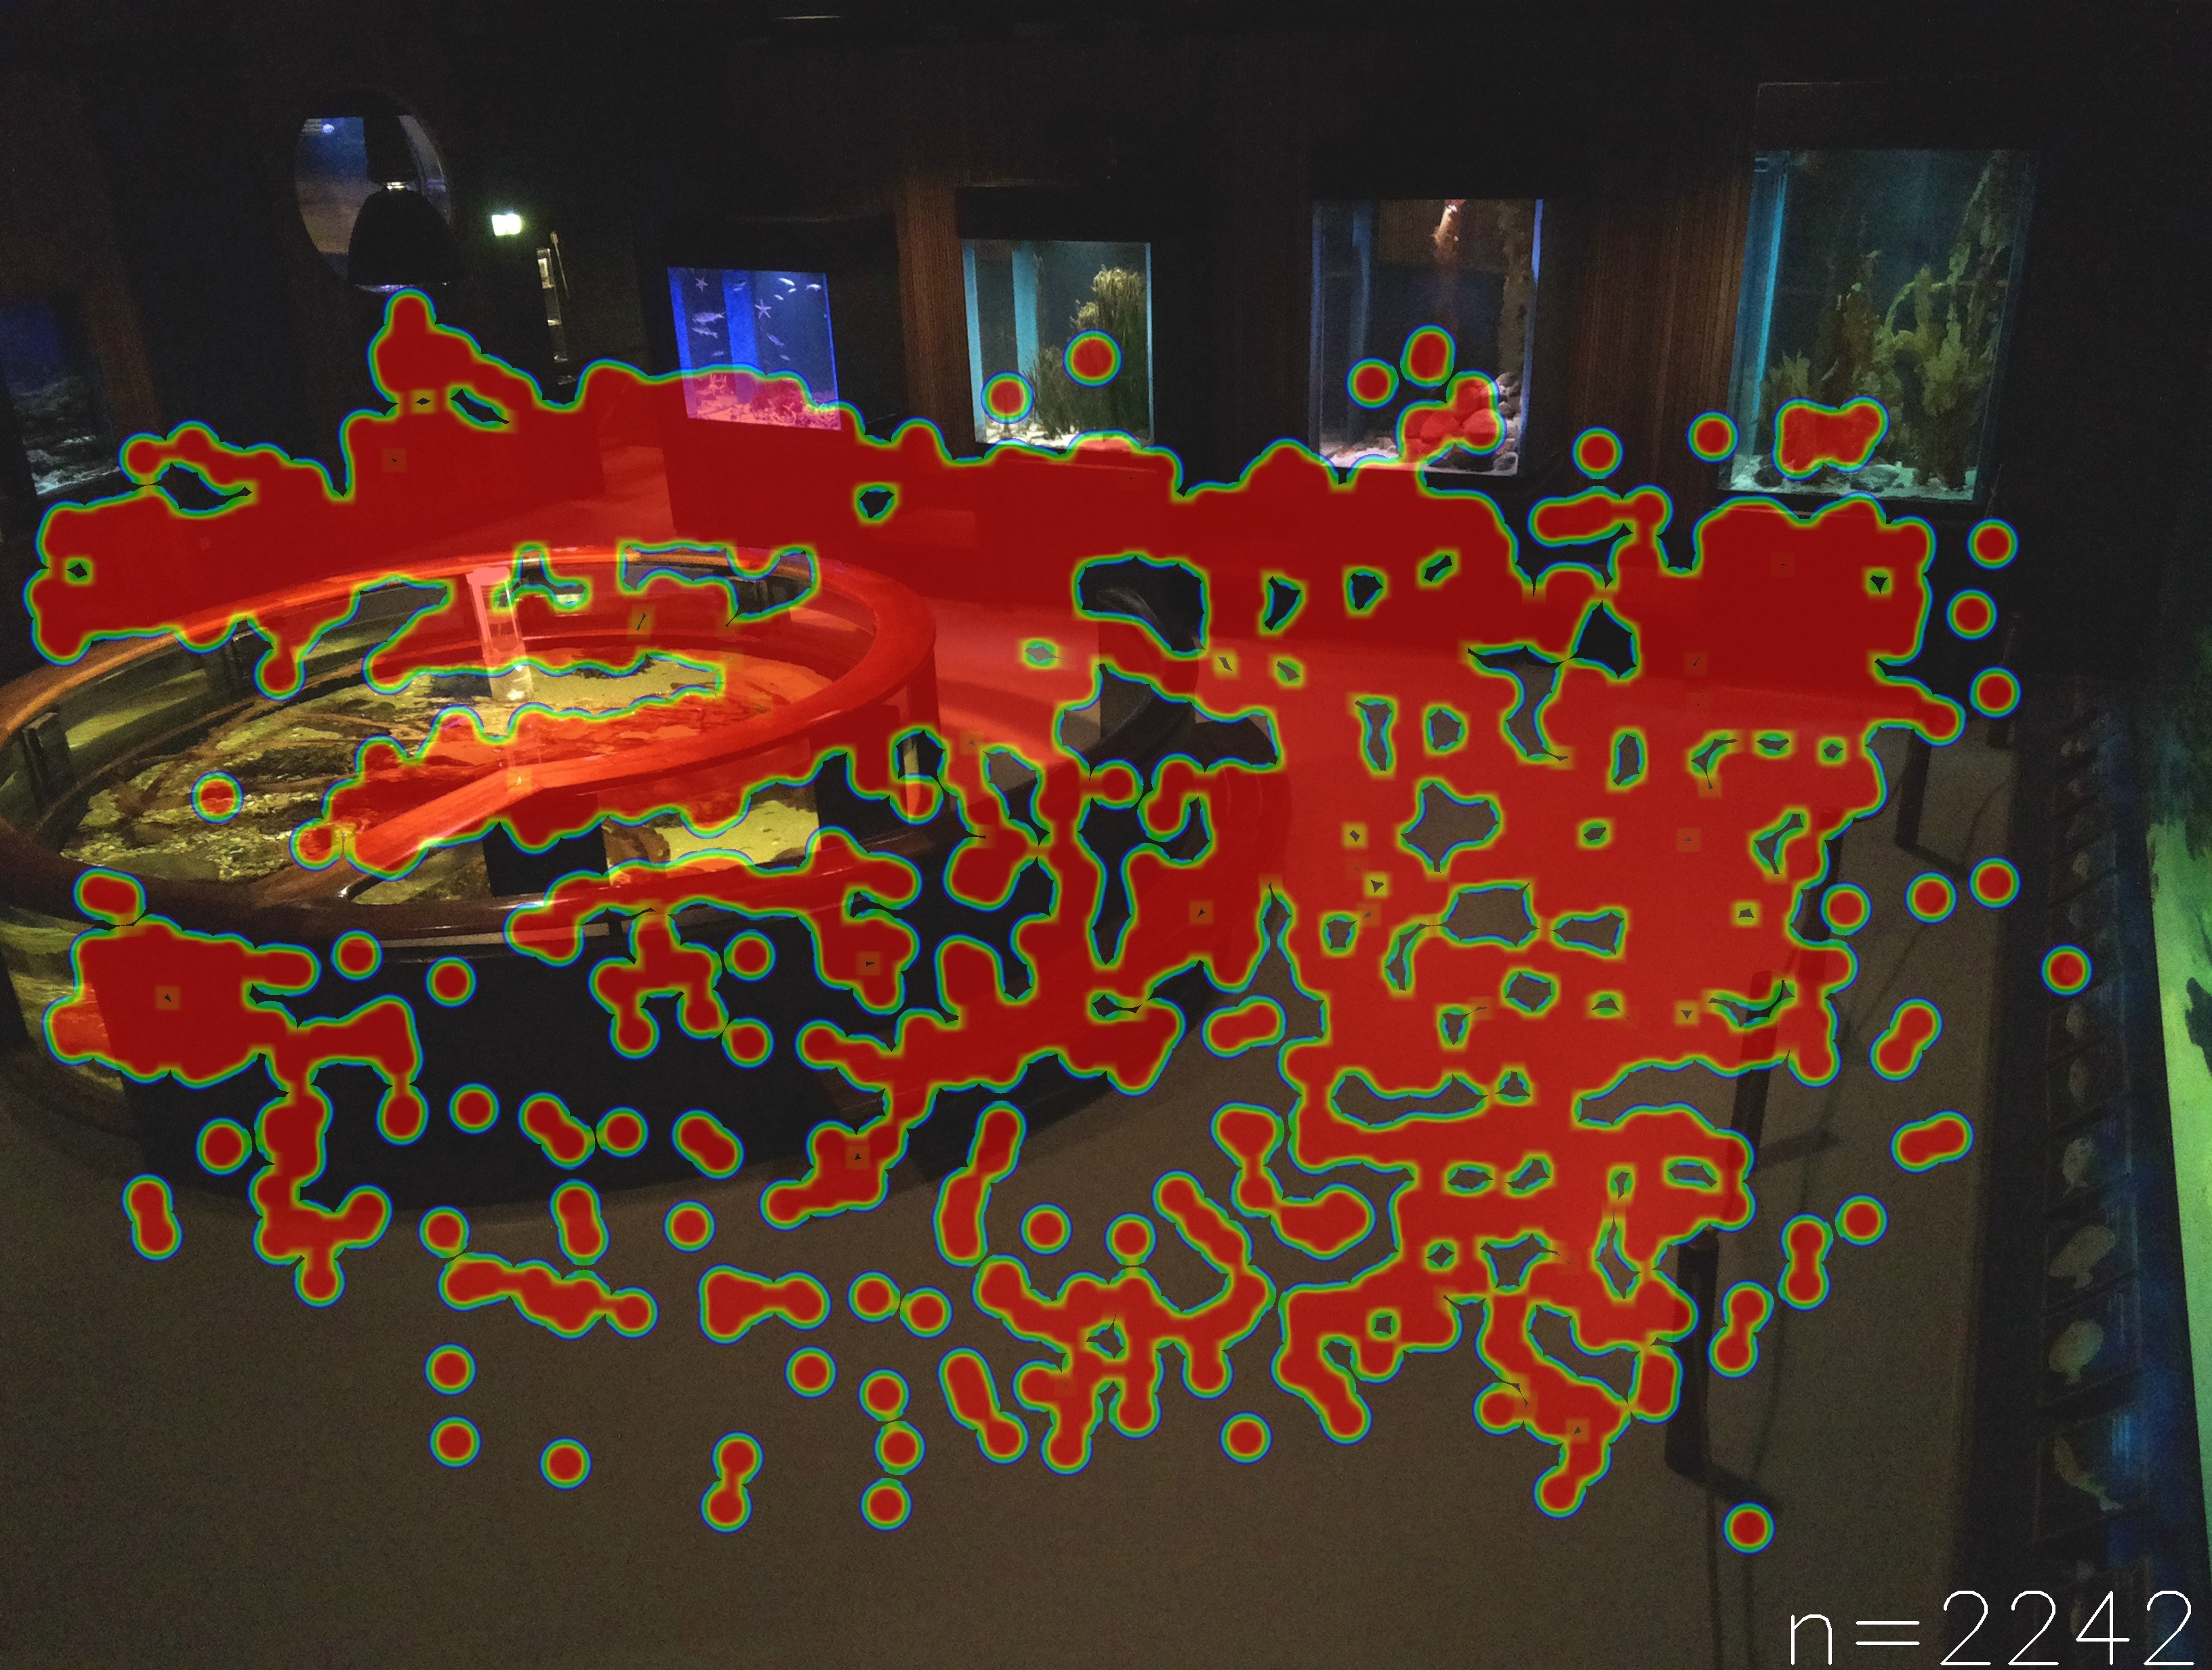
\includegraphics[width=\textwidth]{Images/Analytics/heatmap_center.jpg}
        \caption{Sampled From the \textit{Center} of Detections}
    \end{subfigure}
    \hfill
    \begin{subfigure}{0.475\textwidth}
        \centering
        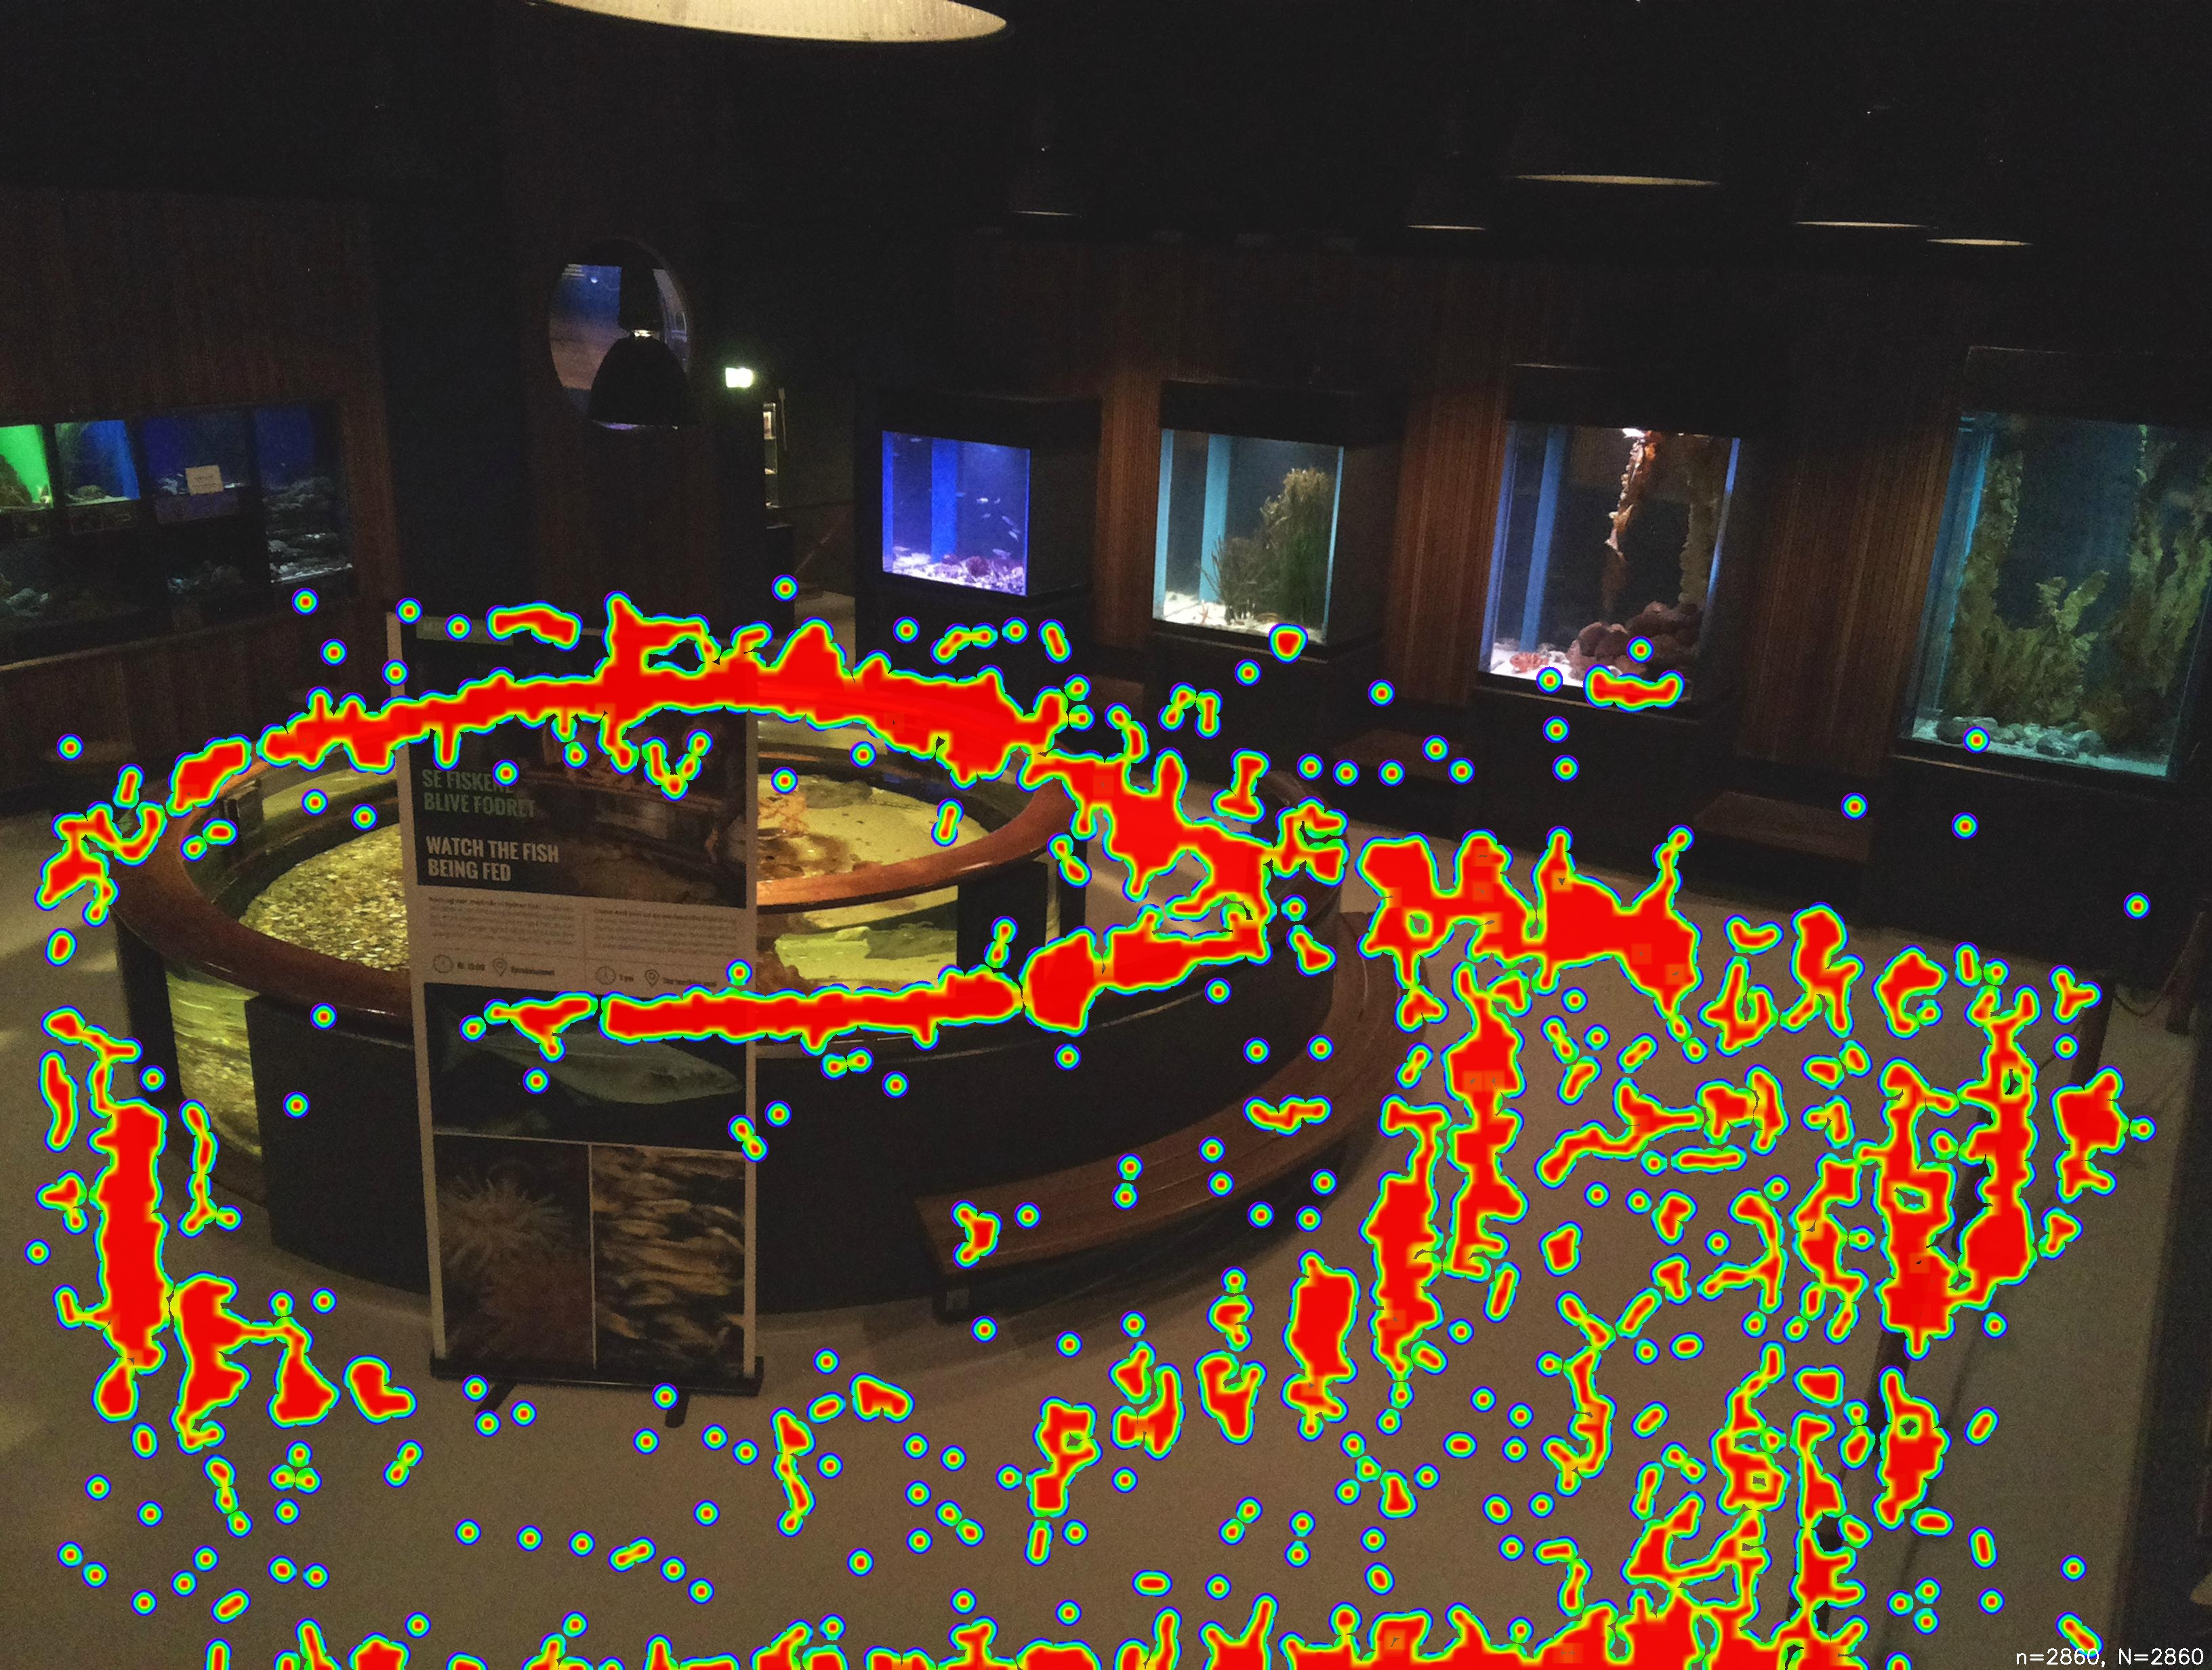
\includegraphics[width=1\textwidth]{Images/Analytics/heatmap_bottom_center.jpg}
        \caption{Sampled From the \textit{Bottom} of Detections}
    \end{subfigure}
    \caption{Weekly Heat maps: Positions Sampled From Center vs Bottom of Each Detection}
    \label{fig:heat_map_final}
\end{figure}

There's another, more important takeaway from the small modification. While seemingly similar, the heat map sampling detections from the middle of the bounding boxes (\ref{fig:heat_map_final}a) reveal a weakness in our detector which is invisible in the other heat map: the lamp is sometimes classified as a person. On the other hand, the other heat map (\ref{fig:heat_map_final}b) reveal another weakness. The seaweed in the second fish tank from the right is sometimes also classified as a person.   

Apart from revealing weaknesses from the detector models\footnote{These weaknesses in our detector models could be revealed by looking at the annotated images. However, looking at the annotated images is not possible for a on-device processing image-deleting device. In this case, one would need to display/plot the detections onto a base-layer image (heat map), or make use of obfuscation discussed in Section \ref{sec:obfuscation} to illustrate and reveal model weaknesses.}, these heat maps may provide valuable insights with regards to which areas of the facility are being used the most. There may be difficulties, however, in correctly inferring what are the reasons for the variations. For periods less than a day, these variations are likely due to randomness. The more interesting numbers in this context would be to see the total number of visitors throughout the day, which is better visualized in the bar charts in Section \ref{sec:peak_hours}. Two heat maps for separate days are illustrated in Figure \ref{fig:heat_map_daily}.

\begin{figure}[H]
    \centering
    \begin{subfigure}{0.475\textwidth}
        \centering
        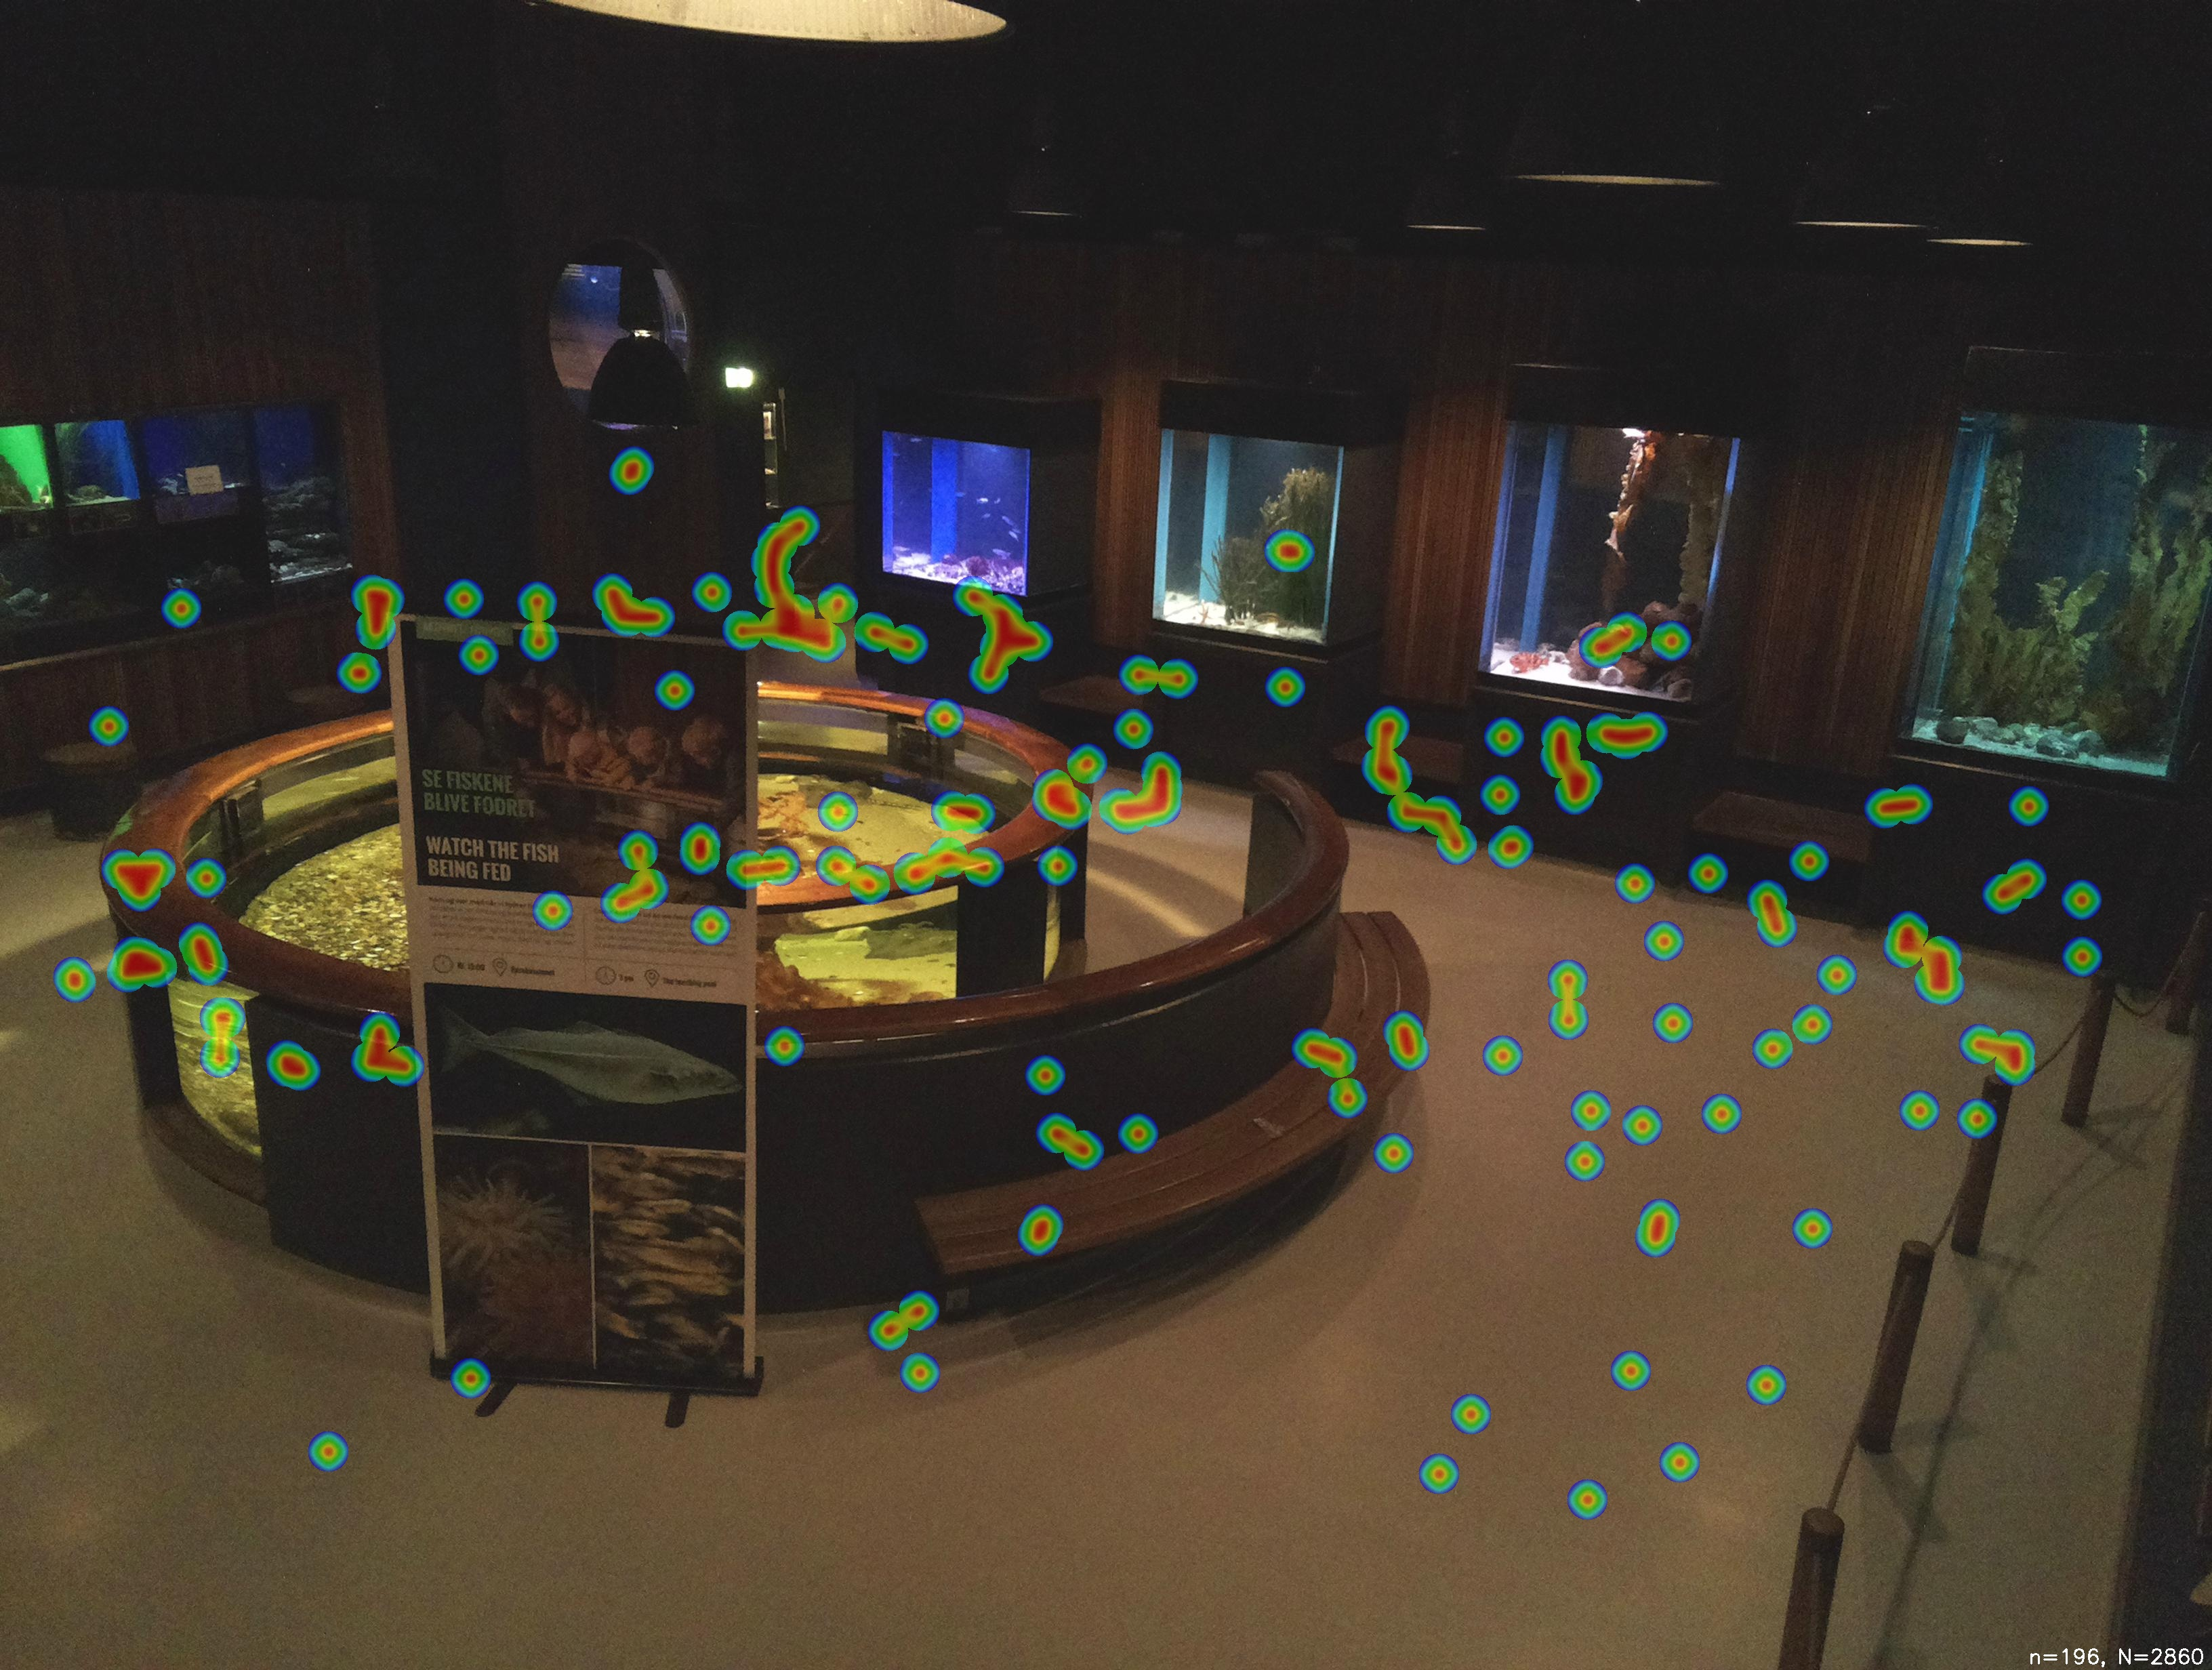
\includegraphics[width=\textwidth]{Images/Analytics/heatmap_day_08052024.jpg}
        \caption{Wednesday 8th of May, 2024}
    \end{subfigure}
    \hfill
    \begin{subfigure}{0.475\textwidth}
        \centering
        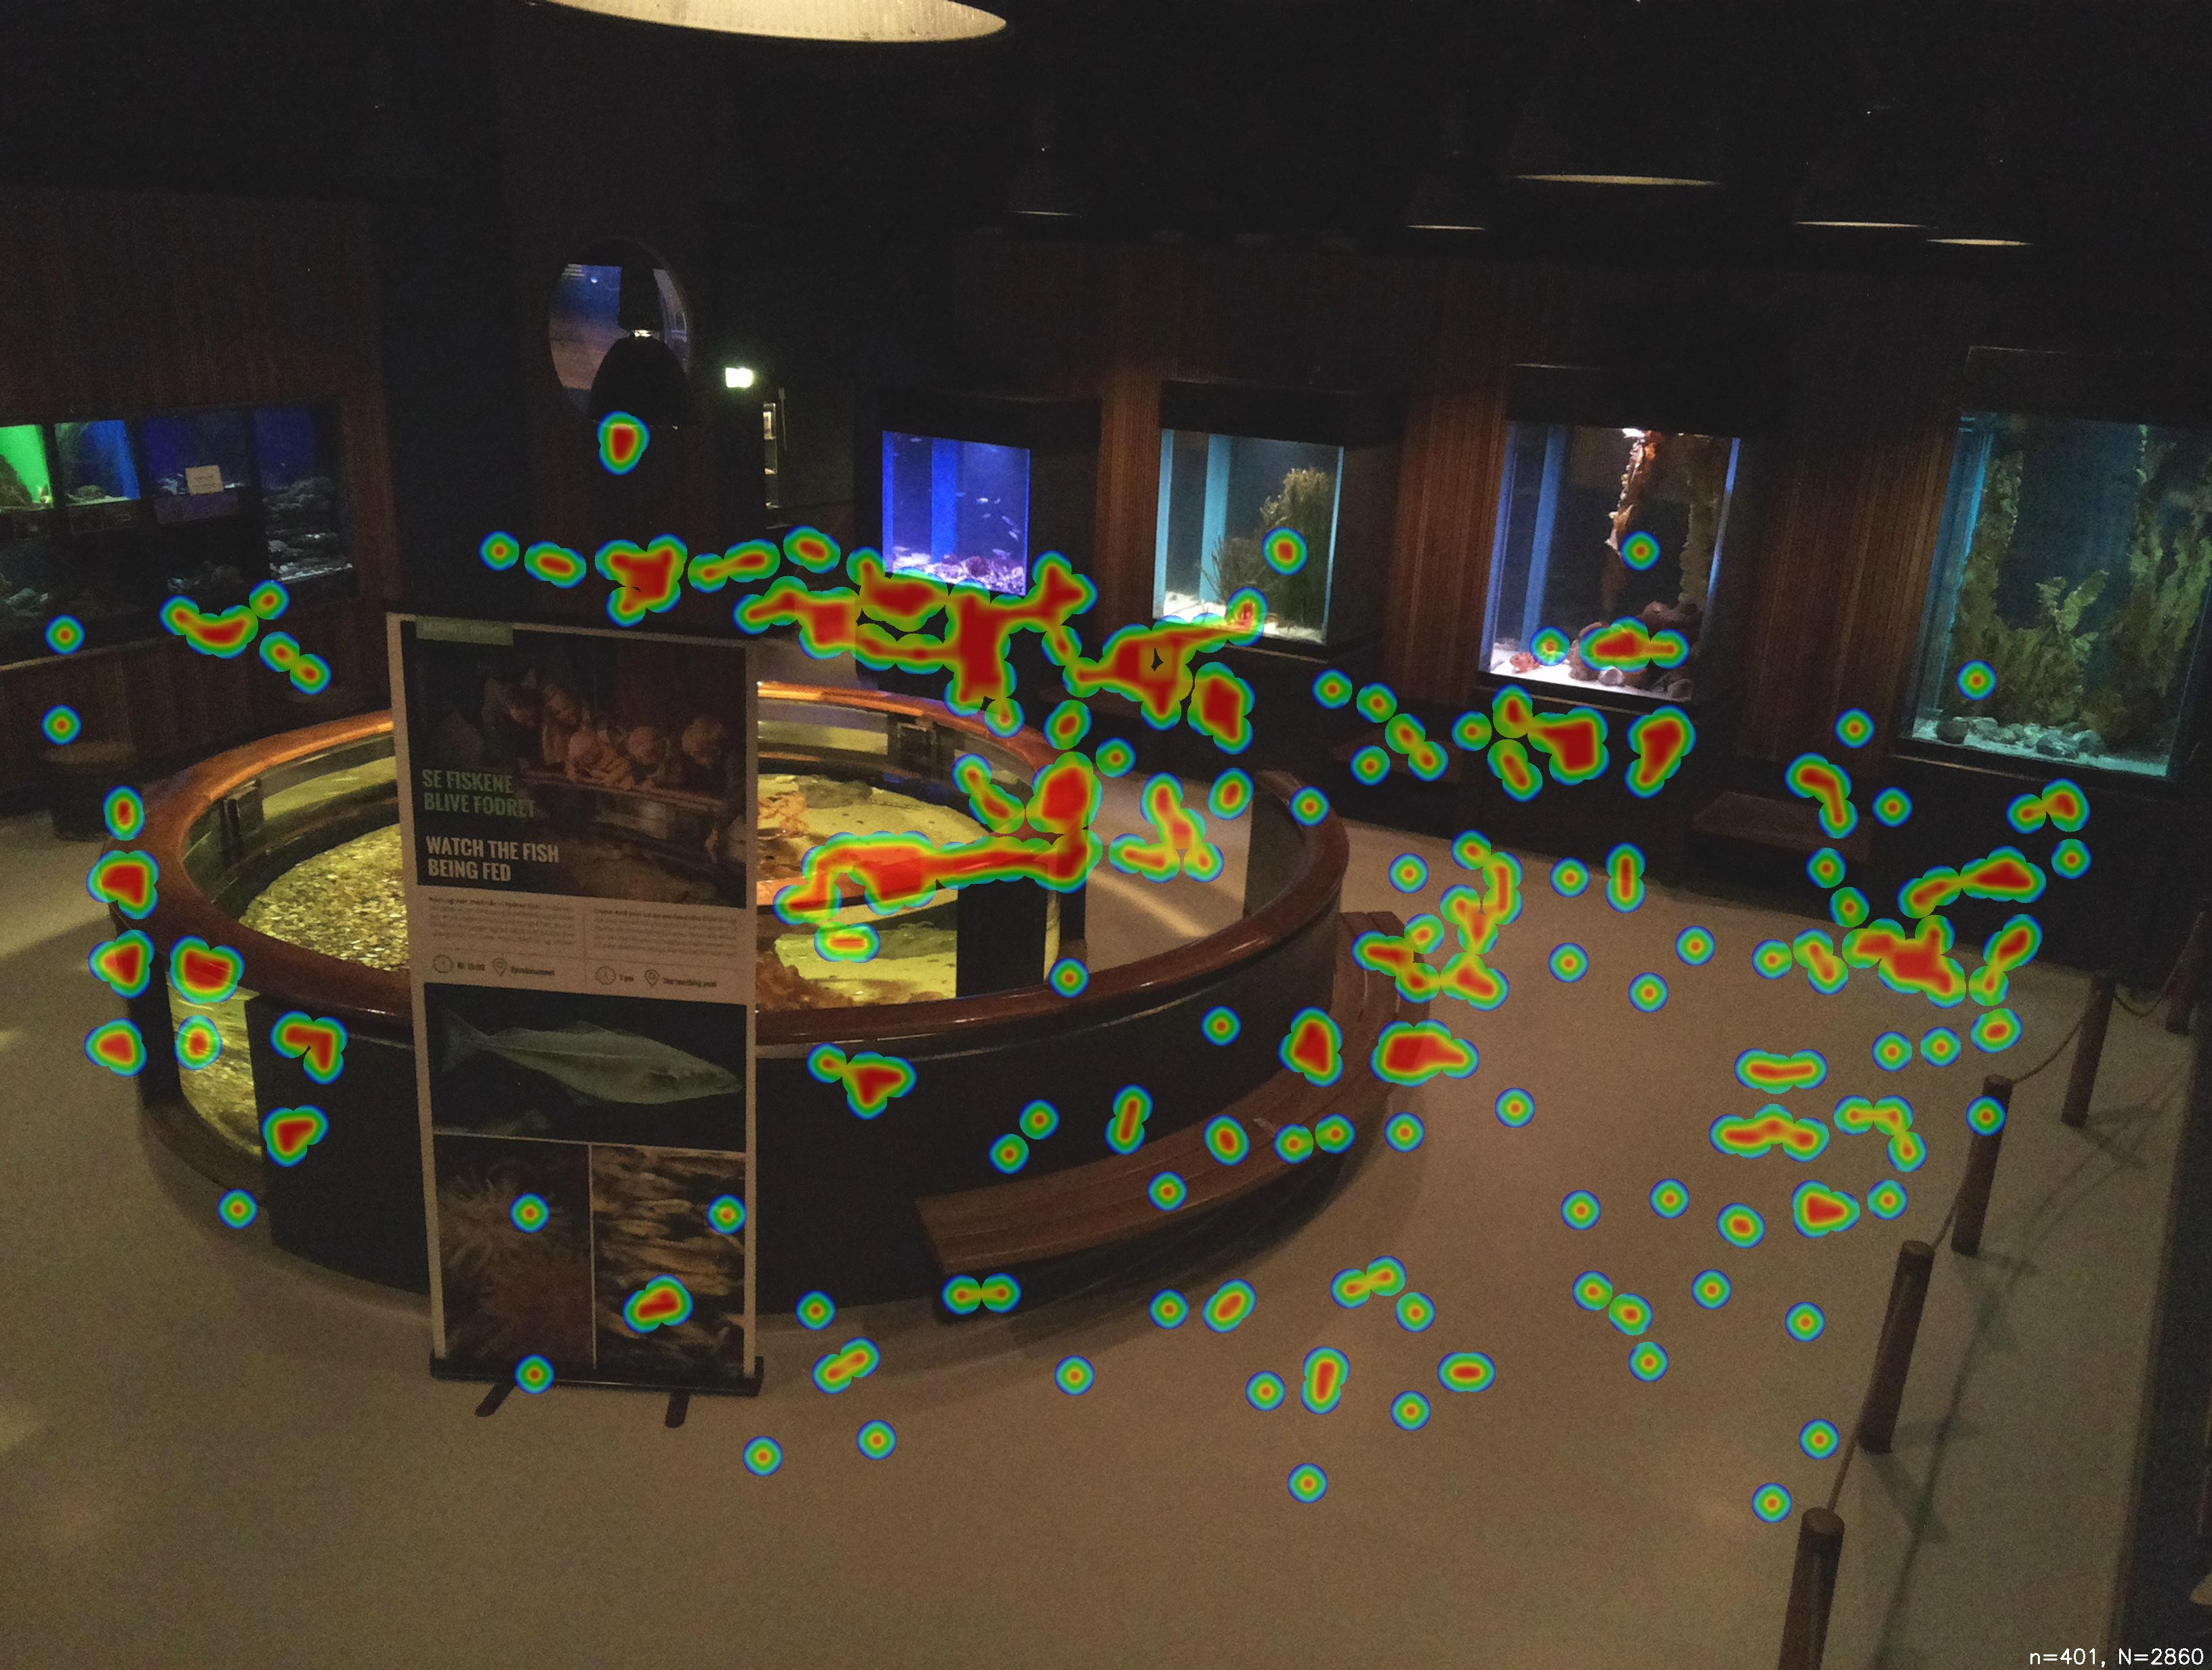
\includegraphics[width=1\textwidth]{Images/Analytics/heatmap_day_11052024.jpg}
        \caption{Saturday 11th of May, 2024}
    \end{subfigure}
    \caption{Daily Heat maps}
    \label{fig:heat_map_daily}
\end{figure}

Heat maps may also visualize the hours throughout a day, accumulating all data for a specific time period each day to see if the visitor engagement changes based on the time. This is one example of introducing a variable, namely the time of day, to filter the detections. For an area where other variables such as the temperature, the noise level or the weather is also known, this could be used instead to filter the detections and illustrate how visitor engagement changes based on these factors. This usage would naturally, require some months-worth of data to be valid. For this project, only a months-worth of positional data has been stored to make the analysis. An illustration of heat maps where the time of day has been used to determine which detections are presented in the heat maps are displayed in Figure \ref{fig:heat_map_time}.

\begin{figure}[H]
    \centering
    \begin{subfigure}{0.475\textwidth}
        \centering
        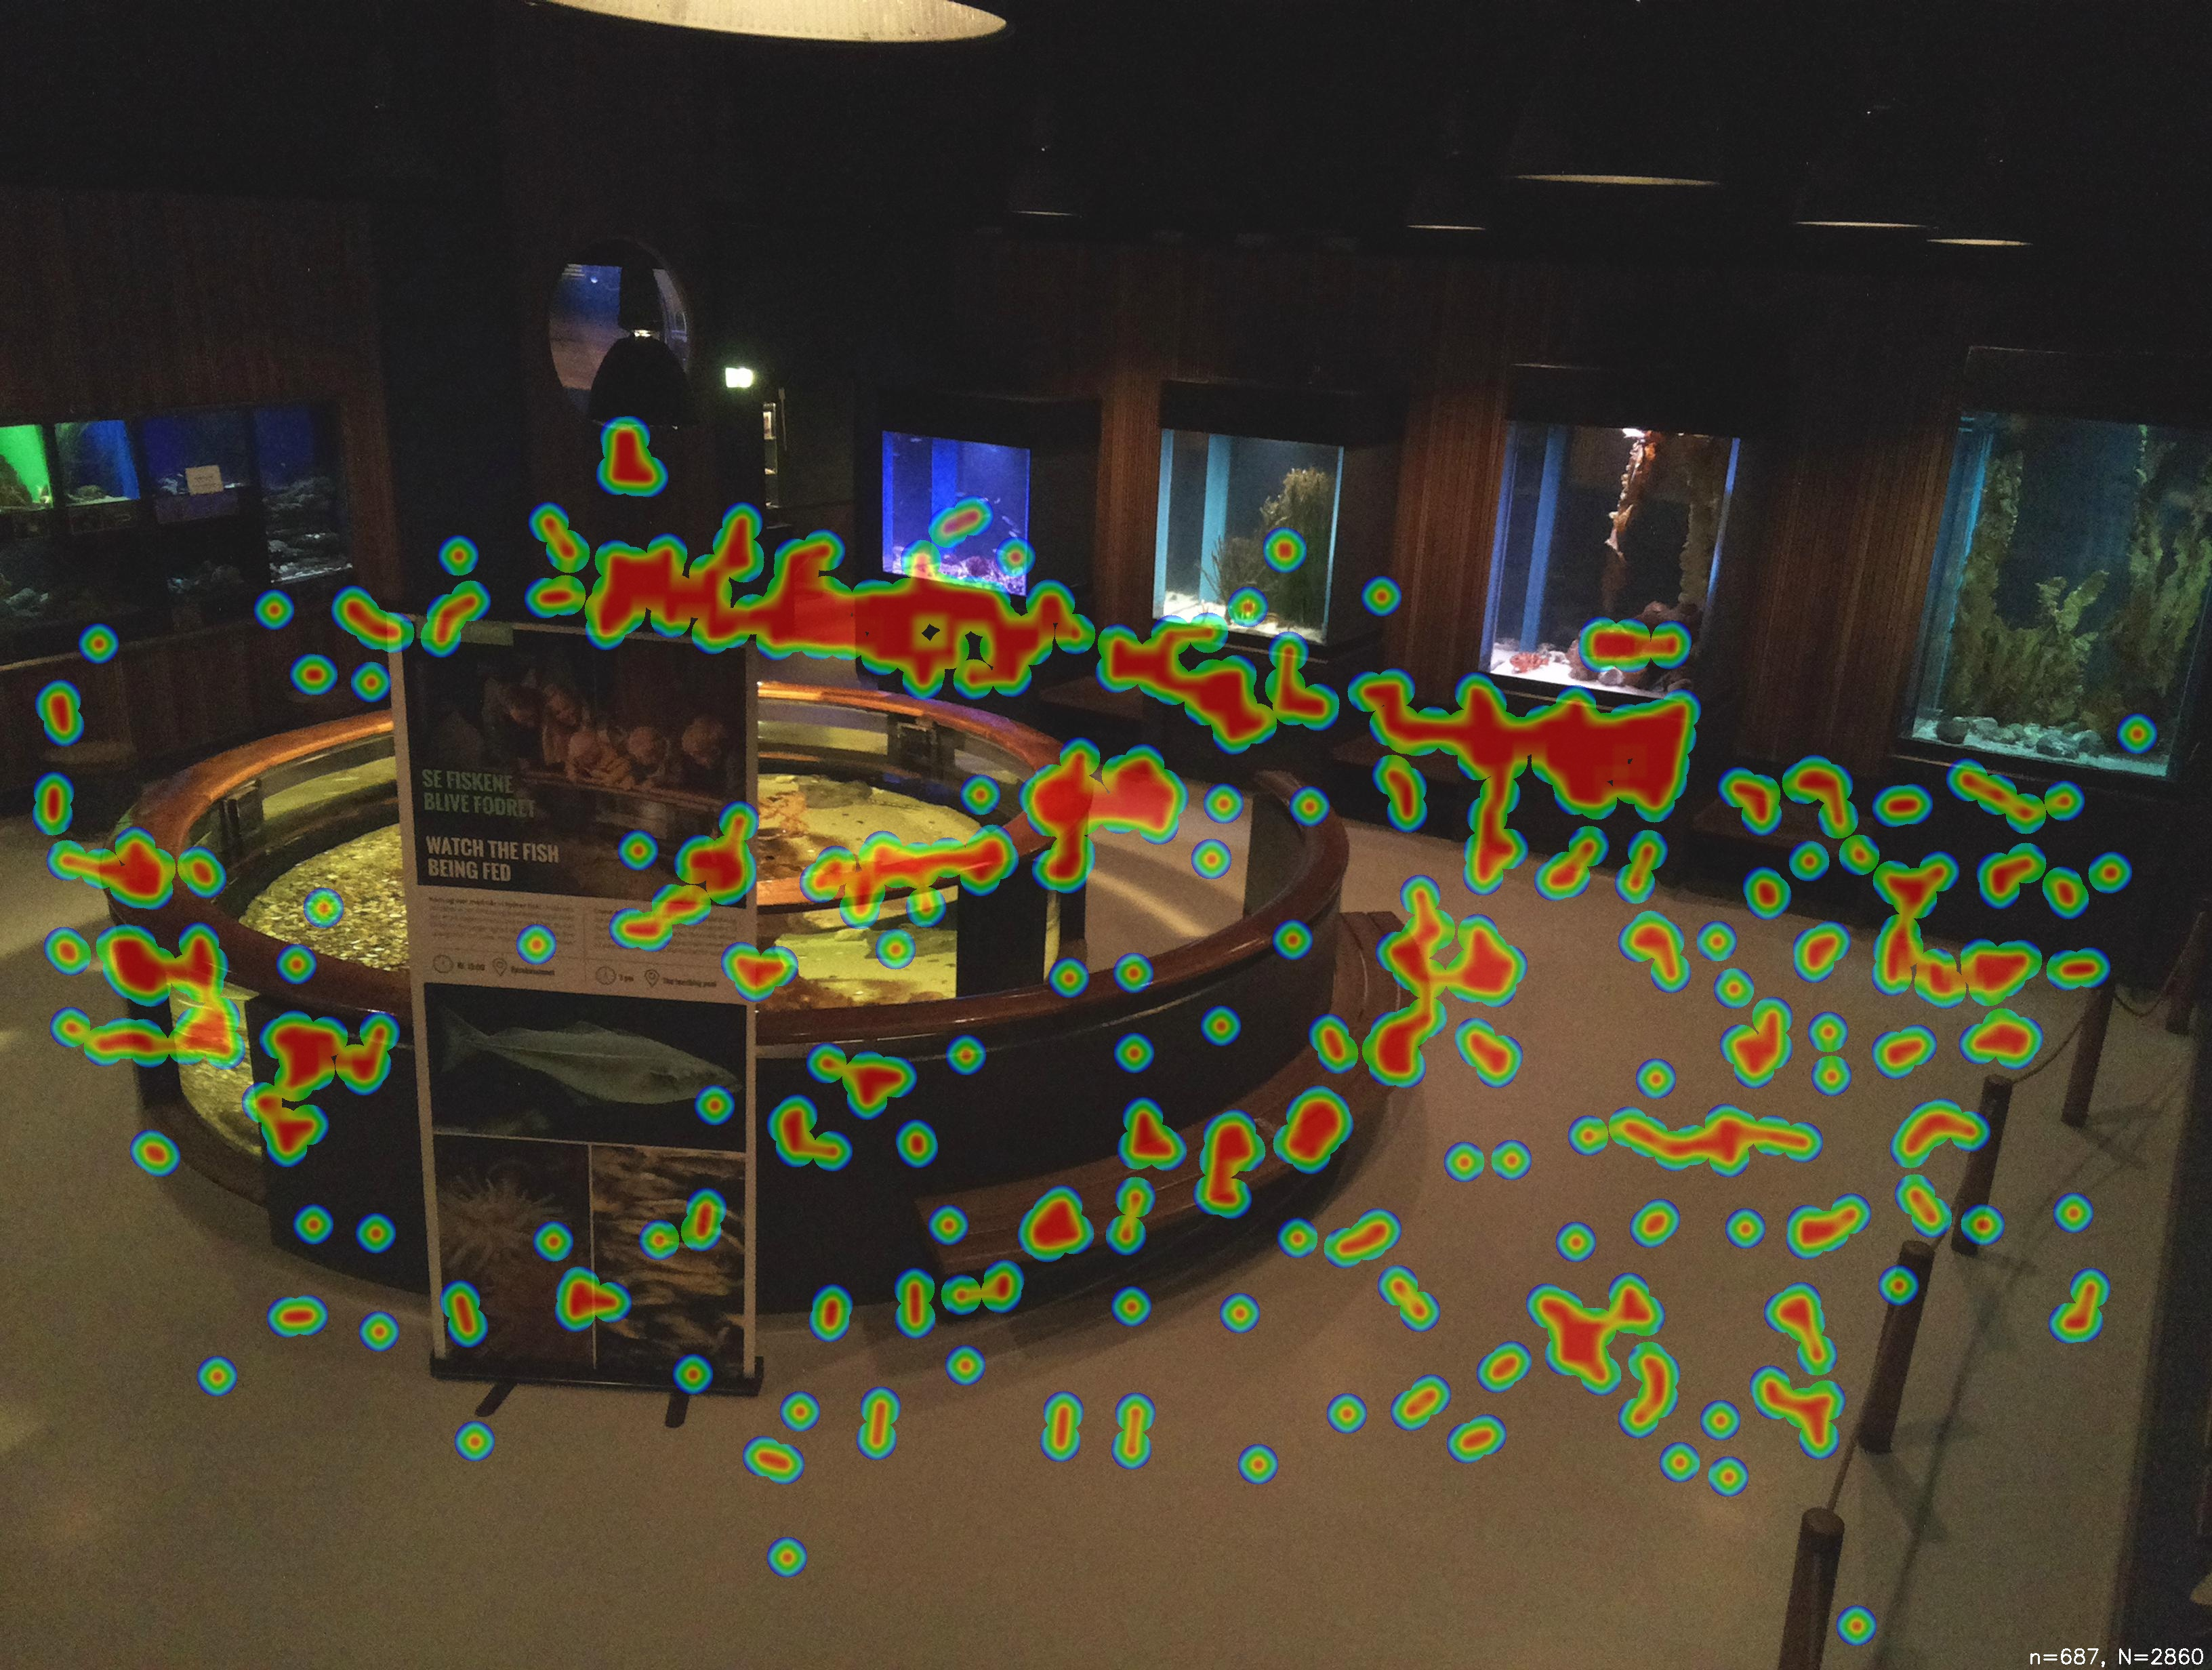
\includegraphics[width=\textwidth]{Images/Analytics/heatmap_time_1300_1400.jpg}
        \caption{13:00-14:00}
    \end{subfigure}
    \hfill
    \begin{subfigure}{0.475\textwidth}
        \centering
        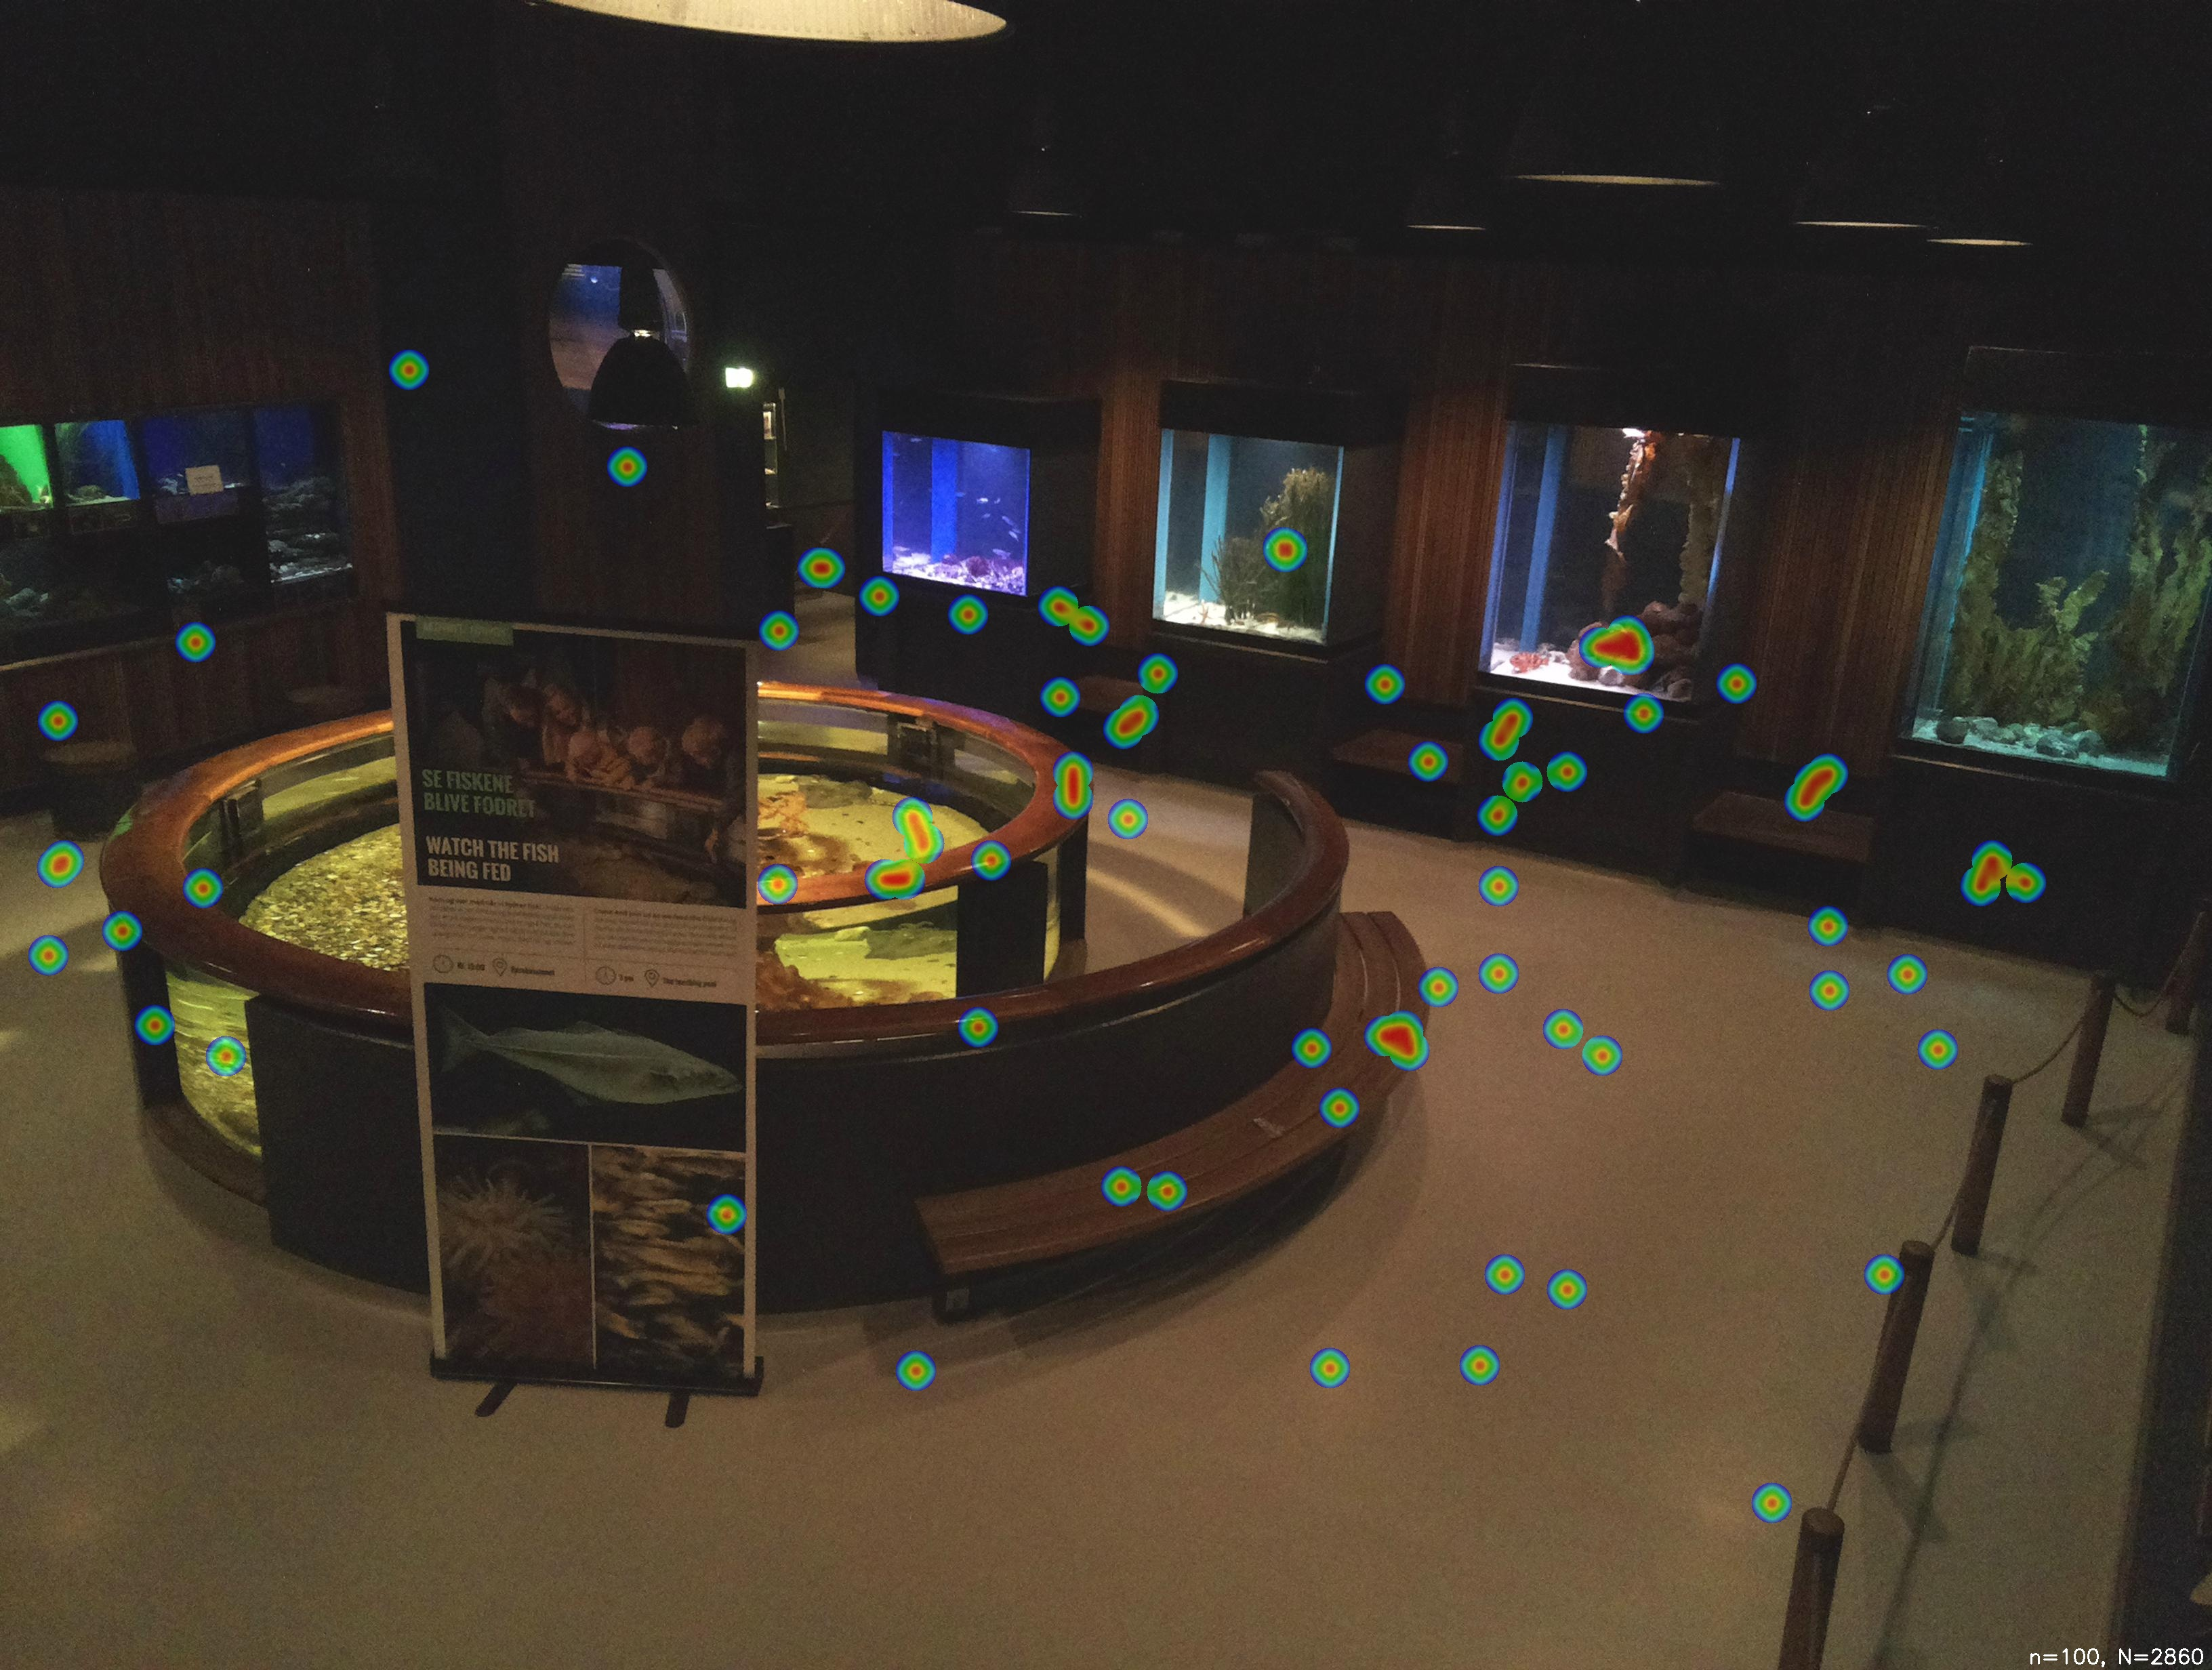
\includegraphics[width=\textwidth]{Images/Analytics/heatmap_time_1600_1700.jpg}
        \caption{16:00-17:00}
    \end{subfigure}
    \caption{Hourly Heat map}
    \label{fig:heat_map_time}
\end{figure}

The heat maps in Figure \ref{fig:heat_map_time} reveal another use case for heat maps. The relative difference between the two heat maps is likely due to randomness, but with a larger number of detections one might be able to look for patterns. This could be that the heat map for 13:00-14:00 could show a higher number of detections in front of the fish tanks, while the heat map for 16:00-17:00 could show a higher number of detections on the benches. This could have easily been overlooked, had a manager of the museum only passed through the museum in the day and never in the evenings, resulting in him not thinking so many benches were neccessary. 

The project experiment with the devices in the aquarium lasted for the entire month of May, and heatsmaps from all of the gathered data are displayed in Figure \ref{fig:heat_map_month}. 

\begin{figure}[H]
    \centering
    \begin{subfigure}{0.475\textwidth}
        \centering
        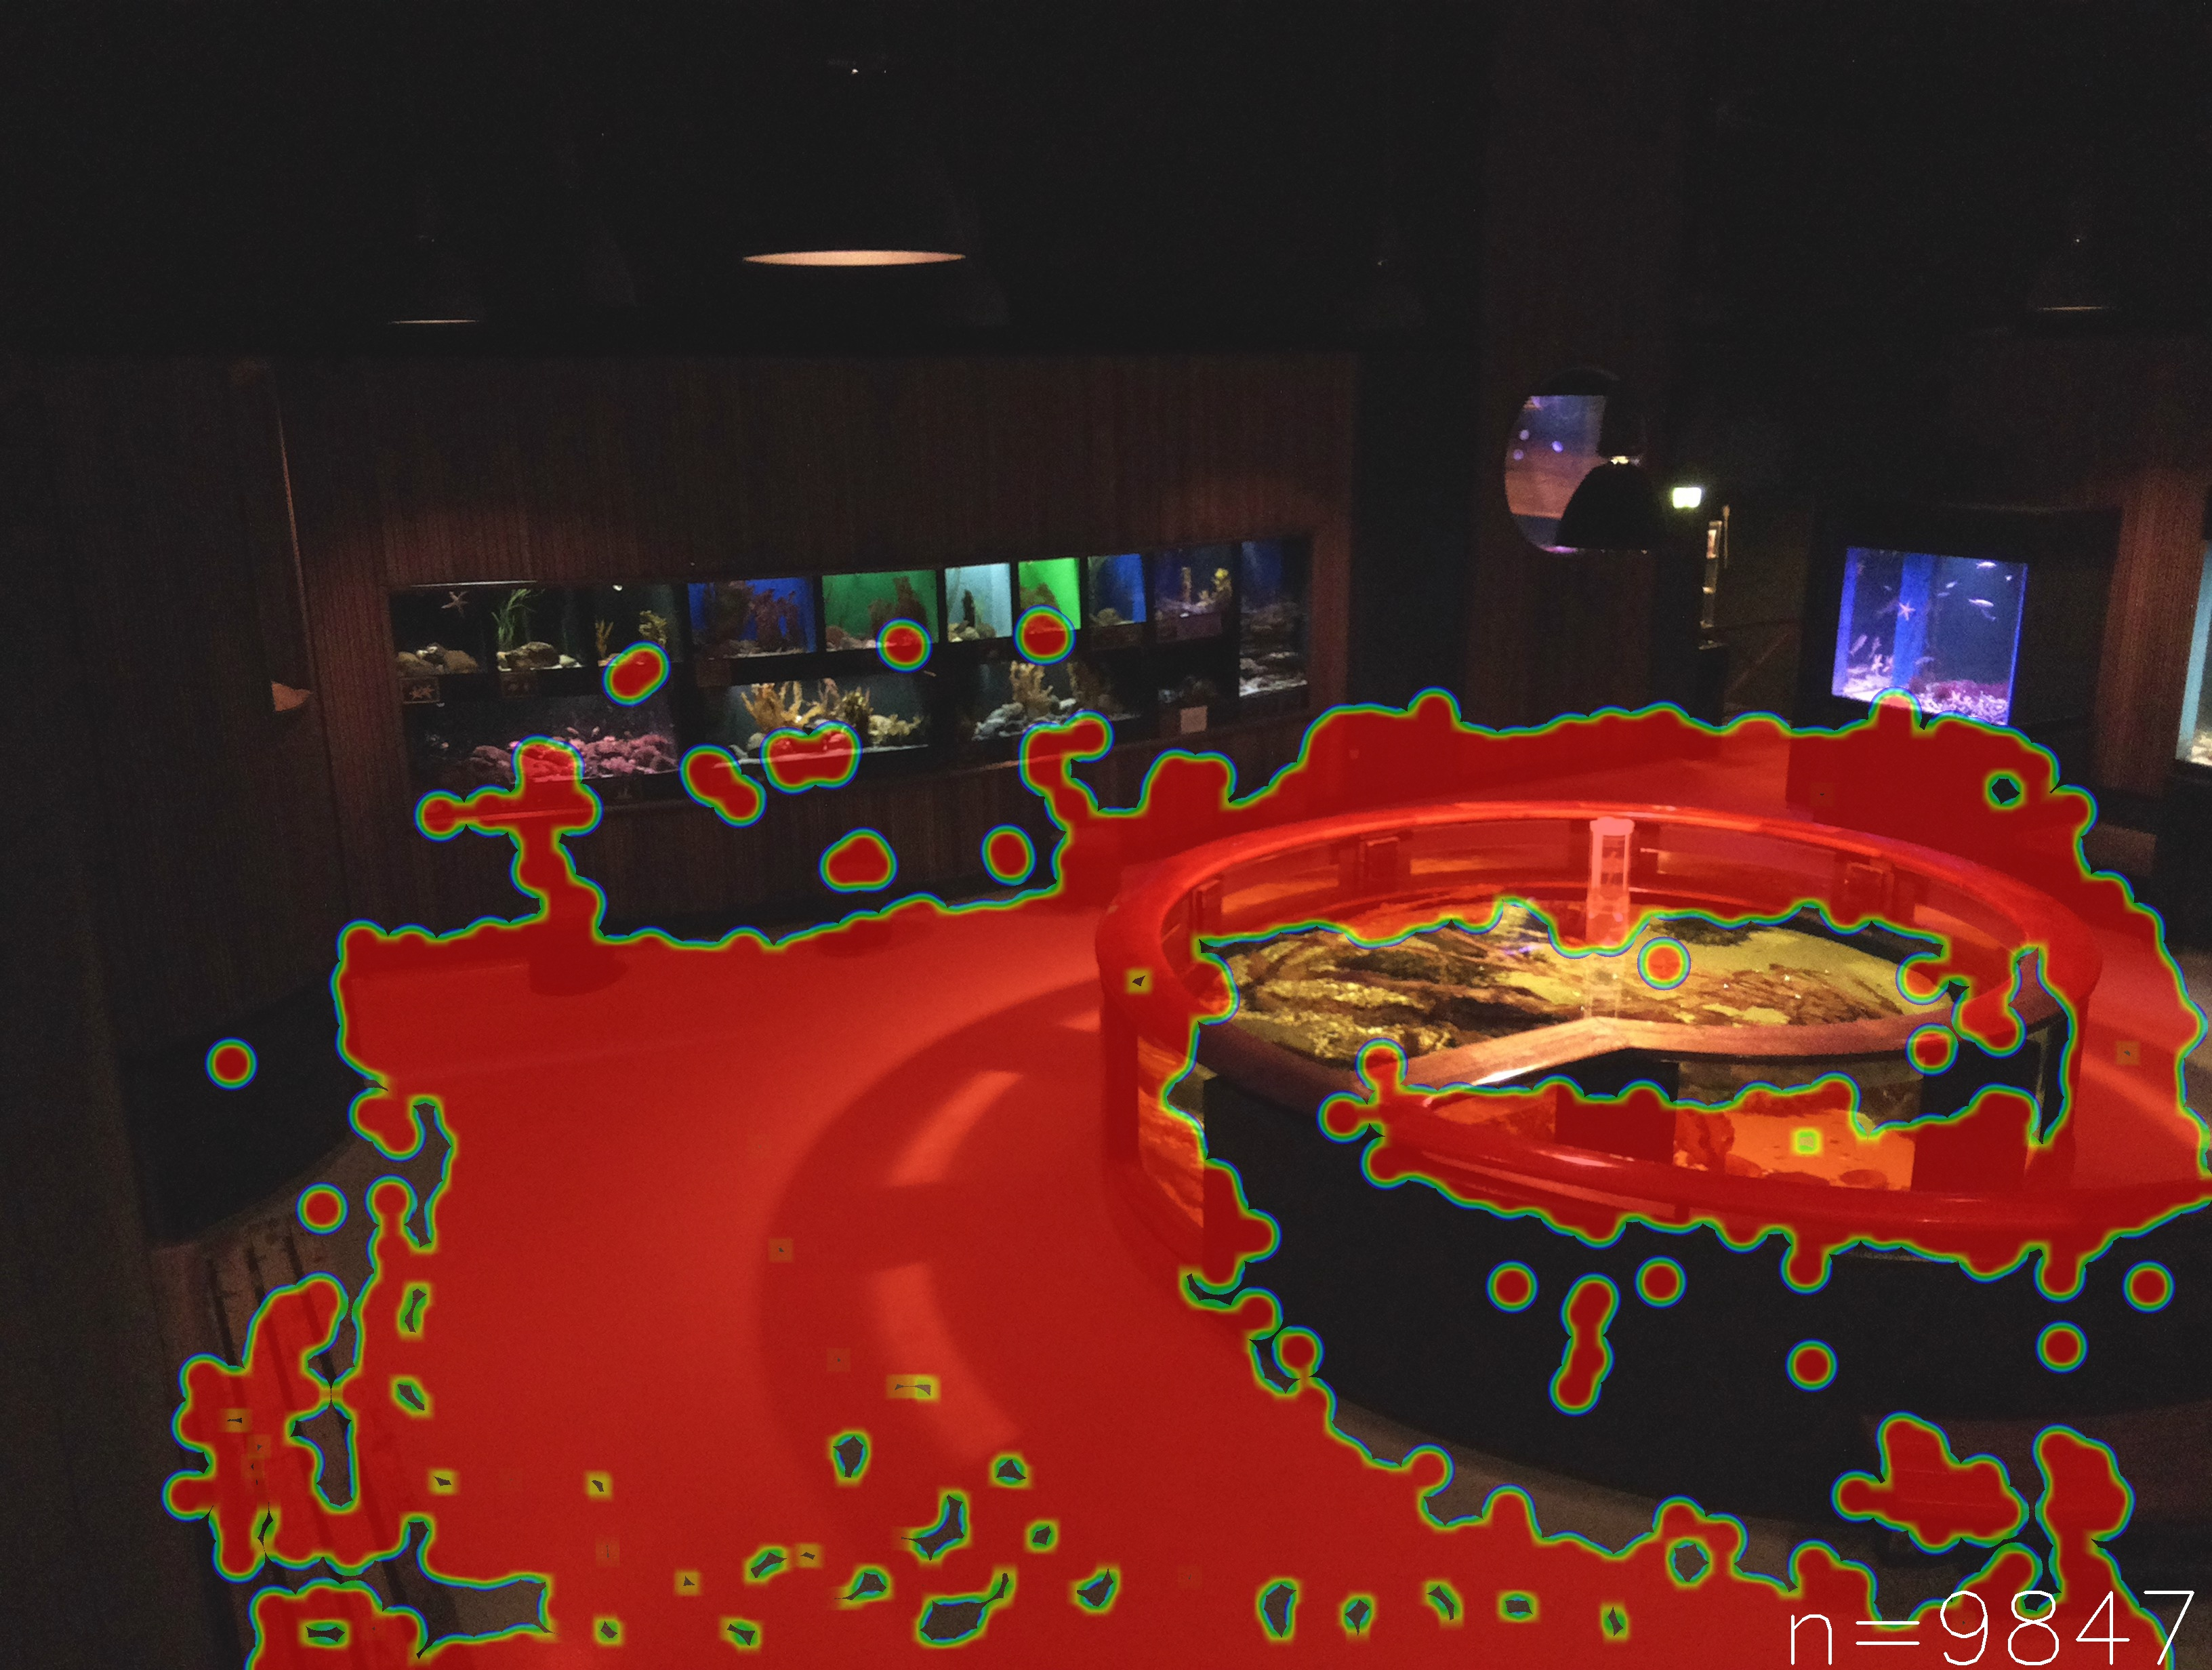
\includegraphics[width=\textwidth]{Images/Analytics/heatmap_left_all.jpg}
        \caption{Left, n=9847}
    \end{subfigure}
    \hfill
    \begin{subfigure}{0.475\textwidth}
        \centering
        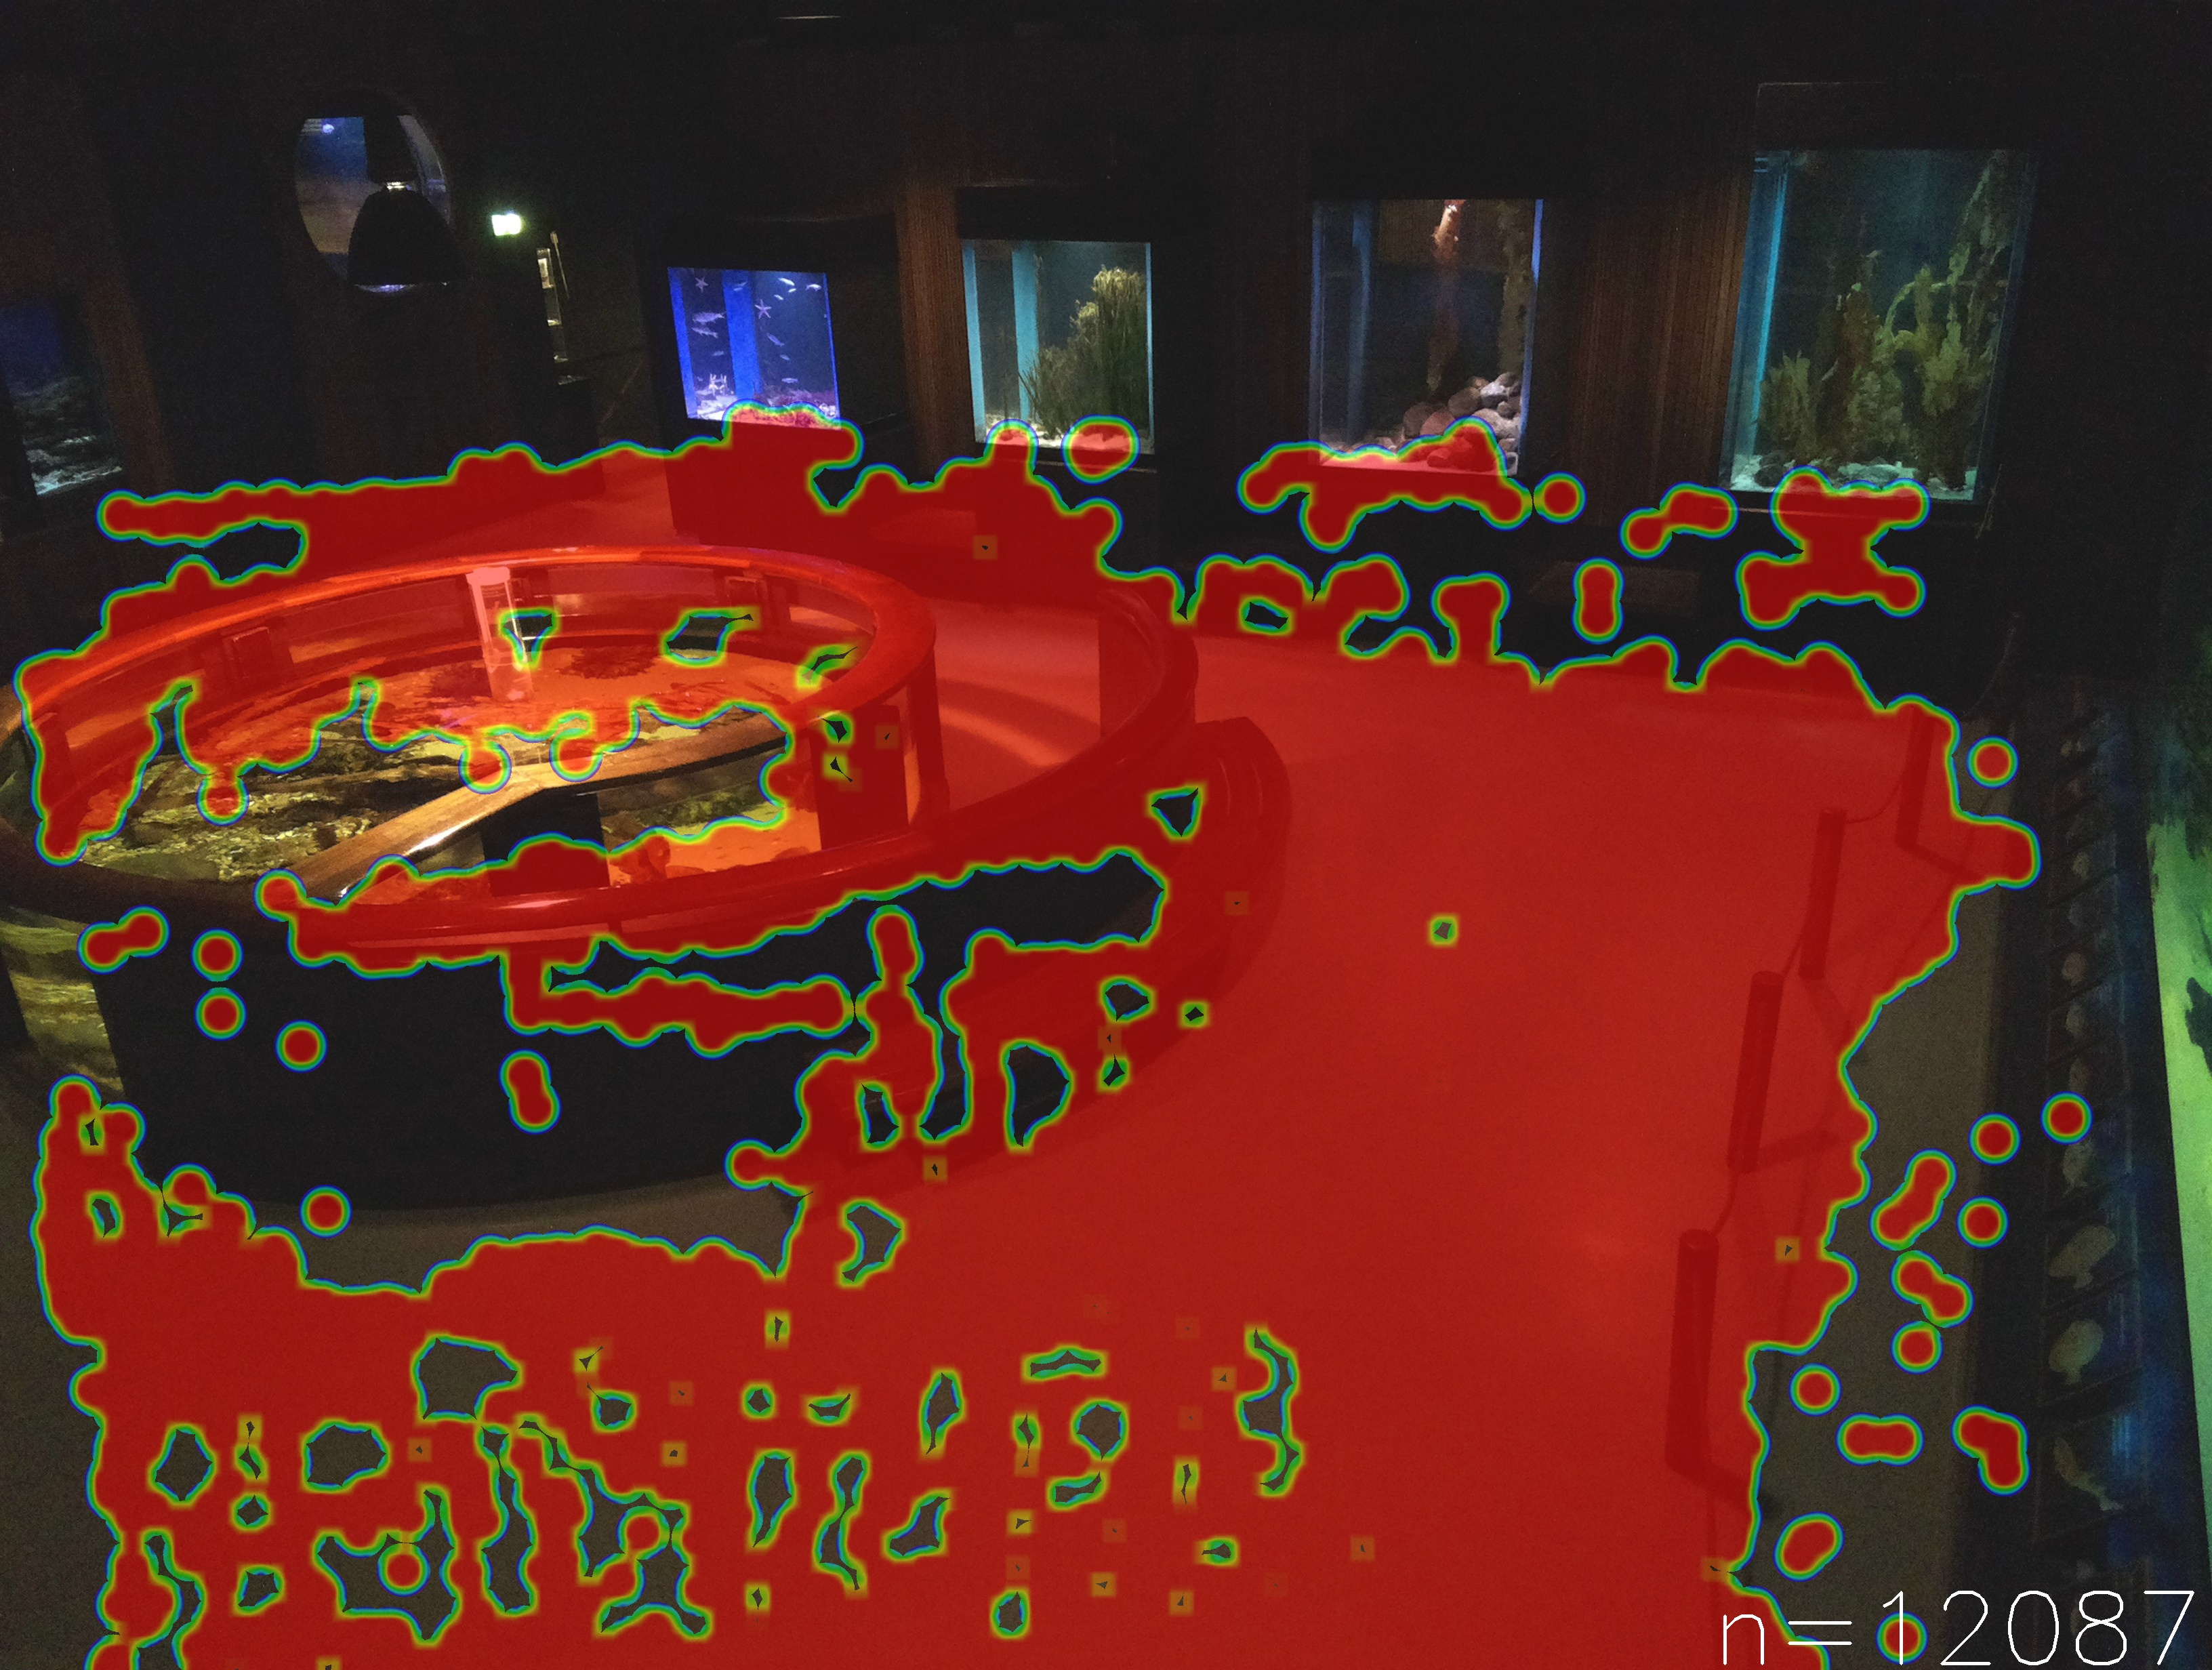
\includegraphics[width=\textwidth]{Images/Analytics/heatmap_right_all.jpg}
        \caption{Right, n=12087}
    \end{subfigure}
    \caption{Monthly Heat map}
    \label{fig:heat_map_month}
\end{figure}

From the heat maps in Figure \ref{fig:heat_map_month}, we can clearly understand the need to filter the data in one of the proposed ways to gather more insightful information. 

\subsubsection{Visitation Count Bar Charts}
\label{sec:peak_hours}
Another tool is to analyze the average number of detected persons per hour. This provides insights into room utilization during different times of the day. Figure \ref{fig:peak_hours} provides an easy to grasp representation of what the peak hours of the aquarium has been. The figure displays that most visitors are in the aquarium from 13:00-13:59. This is not unlikely, as it is the time of the day the aquarium staff feeds the fish. It is also possible to see that the first hour after opening is quite busy, while the last hour from 16:00-16:59 is the hour with the least amount of visitors. The numbers in Figure \ref{fig:peak_hours} are subject to the previously described uncertainty of the model in inferring person localizations.

\begin{figure}[H]
	\centering
	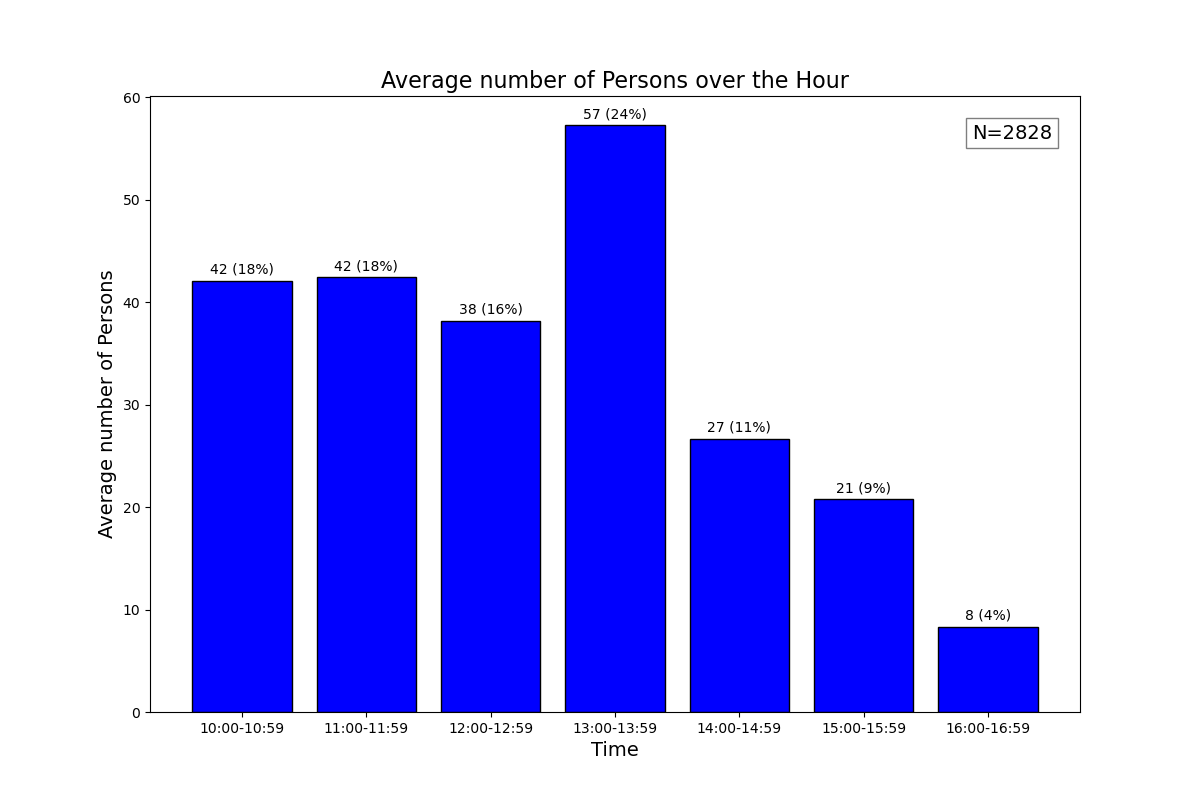
\includegraphics[width=1\textwidth]{Images/Analytics/peak_hours.png}
	\caption{Peak Hours Analysis}
    \label{fig:peak_hours}
\end{figure}

Some insights may be extrapolated from this data. For instance, a lower number of detections during early opening hours, despite high visitor entry, could indicate that the room temperature is not yet optimal, affecting visitor comfort. This hypothesis could be tested by using the number of visitors as the dependent variable and adjust the room temperature to see the effects. In the absence of other confounding variables\footnote{Removing all other confounding variables from a real world setting may be a very difficult task. To do so, one must collect data over a long time period in order to average out the random events and factors that may influence the experiment.}, this could be an interesting causal relationsship to investigate to infer the perfect room temperature. However, due to the requirement in such an investigation for the high volume of data to rule out the possibility of randomness confounding the results, this investigation is likely unrealistic.

Further, comparing visitor detections of summer vs winter months, normalized for the total visitors in the facility, could provide deeper insights. It would enable the possibility of gauging the relative popularity of different areas. Indoor environments, typically maintained at constant temperatures, might offer different levels of comfort compared to the naturally fluctuating conditions of outdoor areas. More data visualization future work potential avenues are discussed in the Future Works section. 

Understanding these dynamics can guide decisions on environmental controls, such as adjusting heating levels to enhance visitor comfort and potentially increase engagement in specific areas of the facility. Such adjustments could directly influence the overall visitation experience, making the whole facility more favorable for a visit regardless of seasonal factors.

A hypothesis was formed during the image capture process by observing the few visitors during the final opening hours of the aquarium. Most late visitors would sit more on the bench, rather than walk and run around the room like many of the earlier visitors would. This is a find that the heat map could have revealed, had it been the case. However, the data-driven visualization (the heat maps), tell us a different story. 

\subsubsection{Data Visualization Future Directions}
Through the development of more sophisticated models, possible future use cases for the technology could be to develop a model to segment the users based on their age group. This could provide graphs to infer e.g. that children are most represented early in the day, and this data could thus be used to have children activities when most of the user group are present to hit the biggest audience. One could also use the data to have children-activities in the afternoon to draw more young visitors to the unpopular visitation hours. The age groups would most succintly expressed as different colored bars in a barchart.  